% Seminarul 10: Modele în spațiul stărilor, filtrul Kalman și modele Markov switching
% Serii de timp -- Programele de licență Informatică economică și Cibernetică economică, Academia de Studii Economice din București
% GENERAT de latex/build_seminar10.py -- modificați generatorul, nu acest fișier.
% Implicit versiunea pentru studenți; versiunea profesorului este wrapper-ul *_solutions.tex.
\makeatletter\@ifundefined{ifsolutions}{\expandafter\newif\csname ifsolutions\endcsname}{}\makeatother

\newcommand{\coursename}{Serii de timp}
\def\tsalang{ro}
% Preambul comun TSA -- Serii de timp / Time Series Analysis (Beamer, 16:9)
% Același design ca MFM și SFM (preluat din SFM, 5 octombrie 2026). Înainte de % Preambul comun TSA -- Serii de timp / Time Series Analysis (Beamer, 16:9)
% Același design ca MFM și SFM (preluat din SFM, 5 octombrie 2026). Înainte de % Preambul comun TSA -- Serii de timp / Time Series Analysis (Beamer, 16:9)
% Același design ca MFM și SFM (preluat din SFM, 5 octombrie 2026). Înainte de \input{../../latex/preamble} se definește
%   \newcommand{\coursename}{Time Series Analysis}      (EN)
%   \newcommand{\coursename}{Serii de timp}       (RO)  și  \def\tsalang{ro}
% Fișierele .tex se află în EN/Courses, EN/Seminars, RO/Cursuri, RO/Seminarii (două niveluri sub rădăcină).
% Deck-urile sînt generate de latex/build_chapterN.py / build_seminarN.py (vezi latex/tsa_build.py).

\documentclass[9pt, aspectratio=169, t]{beamer}
\providecommand{\coursename}{Time Series Analysis}

% Ensure content fits on slides
\setbeamersize{text margin left=8mm, text margin right=8mm}
% Smaller institute font (title page)
\setbeamerfont{institute}{size=\footnotesize}

%=============================================================================
% THEME AND STYLE CONFIGURATION
%=============================================================================
\usetheme{default}
% Using default theme for clean header/footer control

% Color Palette (matching Redispatch PDF)
\definecolor{MainBlue}{RGB}{26, 58, 110}
\definecolor{AccentBlue}{RGB}{26, 58, 110}
\definecolor{IDAred}{RGB}{205, 0, 0}
\definecolor{DarkGray}{RGB}{51, 51, 51}
\definecolor{MediumGray}{RGB}{128, 128, 128}
\definecolor{LightGray}{RGB}{248, 248, 248}
\definecolor{VeryLightGray}{RGB}{235, 235, 235}
\definecolor{KeynoteGray}{RGB}{218, 218, 218}
\definecolor{SectionGray}{RGB}{120, 120, 120}
\definecolor{FooterGray}{RGB}{100, 100, 100}
\definecolor{Crimson}{RGB}{220, 53, 69}
\definecolor{Forest}{RGB}{46, 125, 50}
\definecolor{Amber}{RGB}{181, 133, 63}
\definecolor{Orange}{RGB}{230, 126, 34}
\definecolor{Purple}{RGB}{142, 68, 173}

% Gradient background (exact Keynote 315° gradient: white to RGB 218,218,218)
\setbeamertemplate{background}{%
    \begin{tikzpicture}[remember picture, overlay]
        \shade[shading=axis, shading angle=315,
        top color=white, bottom color=KeynoteGray]
        (current page.south west) rectangle (current page.north east);
    \end{tikzpicture}%
}
% Fallback solid color for compatibility
\setbeamercolor{background canvas}{bg=}

\setbeamercolor{palette primary}{bg=MainBlue, fg=white}
\setbeamercolor{palette secondary}{bg=MainBlue!85, fg=white}
\setbeamercolor{palette tertiary}{bg=MainBlue!70, fg=white}
\setbeamercolor{structure}{fg=MainBlue}
\setbeamercolor{title}{fg=IDAred}
\setbeamercolor{frametitle}{fg=IDAred, bg=}
\setbeamercolor{block title}{bg=MainBlue, fg=white}
\setbeamercolor{block body}{bg=VeryLightGray, fg=DarkGray}
\setbeamercolor{block title alerted}{bg=Crimson, fg=white}
\setbeamercolor{block body alerted}{bg=Crimson!8, fg=DarkGray}
\setbeamercolor{block title example}{bg=Forest, fg=white}
\setbeamercolor{block body example}{bg=Forest!8, fg=DarkGray}
\setbeamercolor{item}{fg=MainBlue}

% Footer colors (override Madrid theme blue)
\setbeamercolor{author in head/foot}{fg=FooterGray, bg=}
\setbeamercolor{title in head/foot}{fg=FooterGray, bg=}
\setbeamercolor{date in head/foot}{fg=FooterGray, bg=}
\setbeamercolor{section in head/foot}{fg=FooterGray, bg=}
\setbeamercolor{subsection in head/foot}{fg=FooterGray, bg=}

% Bullet styles (apply everywhere including blocks)
\setbeamertemplate{itemize item}{\color{MainBlue}$\boxdot$}
\setbeamertemplate{itemize subitem}{\color{MainBlue}$\blacktriangleright$}
\setbeamertemplate{itemize subsubitem}{\color{MainBlue}\tiny$\bullet$}
\setbeamertemplate{itemize/enumerate body begin}{\normalsize}
\setbeamertemplate{itemize/enumerate subbody begin}{\normalsize}

% Item spacing - compact style
\setlength{\leftmargini}{10pt}       % Level 1: minimal indent
\setlength{\leftmarginii}{10pt}      % Level 2: minimal additional indent
% Compact list spacing (zero extra space before/after lists in blocks)
\makeatletter
\def\@listi{\leftmargin\leftmargini \topsep 0pt \parsep 0pt \itemsep 0pt}
\def\@listii{\leftmargin\leftmarginii \topsep 0pt \parsep 0pt \itemsep 0pt}
\makeatother

\setbeamertemplate{navigation symbols}{}

%=============================================================================
% CUSTOM HEADLINE
%=============================================================================
\setbeamertemplate{headline}{%
    \vskip10pt%
    \hbox to \paperwidth{%
        \hskip0.5cm%
        {\small\color{FooterGray}\renewcommand{\hyperlink}[2]{##2}\insertsectionhead}%
        \hfill%
        \textcolor{FooterGray}{\small\insertframenumber}%
        \hskip0.5cm%
    }%
    \vskip4pt%
    {\color{FooterGray}\hrule height 0.4pt}%
}

%=============================================================================
% CUSTOM FOOTER
%=============================================================================
\usepackage{fontawesome5}

\setbeamertemplate{footline}{%
    {\color{FooterGray}\hrule height 0.4pt}%
    \vskip4pt%
    \hbox to \paperwidth{%
        \hskip0.5cm%
        \textcolor{FooterGray}{\small\coursename}%
        \hfill%
        \raisebox{-0.1em}{%
            \begin{tikzpicture}[x=0.08em, y=0.08em, line width=0.4pt]
                \draw[FooterGray] (0,3) -- (1,4) -- (2,3.5) -- (3,5) -- (4,4) -- (5,6) -- (6,5.5) -- (7,4) -- (8,5) -- (9,7) -- (10,6) -- (11,5) -- (12,6.5) -- (13,8) -- (14,7) -- (15,6) -- (16,7.5) -- (17,9) -- (18,8) -- (19,7) -- (20,8.5) -- (21,10) -- (22,9) -- (23,8) -- (24,9.5);
            \end{tikzpicture}%
        }%
        \hskip0.5cm%
    }%
    \vskip6pt%
}

%=============================================================================
% PACKAGES
%=============================================================================
\usepackage[utf8]{inputenc}
\DeclareUnicodeCharacter{03B1}{\ensuremath{\alpha}}
\usepackage[T1]{fontenc}
\usepackage{amsmath, amssymb, amsthm}
\usepackage{mathtools}
\usepackage{bm}
\usepackage{tikz}
\usetikzlibrary{arrows.meta, positioning, shapes, calc, decorations.pathreplacing, shadings}
\usepackage{booktabs}
\usepackage{multirow}
\usepackage{array}
\usepackage{graphicx}
\usepackage{animate}
\usepackage{hyperref}
\usepackage{colortbl}
\usepackage{listings}
\lstset{language=Python, basicstyle=\ttfamily\scriptsize, keywordstyle=\color{MainBlue}\bfseries,
  commentstyle=\color{Forest}, stringstyle=\color{Crimson}, breaklines=true,
  frame=none, backgroundcolor=\color{VeryLightGray}, xleftmargin=2mm}
\hypersetup{colorlinks=true, linkcolor=MainBlue, urlcolor=MainBlue}
\graphicspath{{../../logos/}{../../charts/}{../../photos/}}
\usepackage{xcolor}
\hfuzz=2pt  % Suppress tiny overfull warnings (<2pt)
\vfuzz=2pt  % Suppress tiny vertical overfull warnings (<2pt)
% \mathrm in the sans-serif family of the slides (beamer resets \mathrm to the serif family at \begin{document};
% this hook runs after beamer's, so WN, Var, RMSE, ... in formulas match the surrounding text)
% Bold vectors and matrices in the same sans-serif family: \mathbf{A} in sans bold (beamer's own \mathbf came out in
% medium weight), and the bold upright Greek capitals of \boldsymbol / \bm (\bSigma, \bPhi, \boldsymbol{\Theta}) in
% cmss bold: bm.sty fixes its "boldoperators" font when it is loaded (serif cmbx), before beamer switches the
% operators to cmss, so it is reset here.
\AtBeginDocument{%
  \SetMathAlphabet{\mathrm}{normal}{\encodingdefault}{\sfdefault}{\mddefault}{n}%
  \SetMathAlphabet{\mathrm}{bold}{\encodingdefault}{\sfdefault}{bx}{n}%
  \SetMathAlphabet{\mathbf}{normal}{\encodingdefault}{\sfdefault}{bx}{n}%
  \SetMathAlphabet{\mathbf}{bold}{\encodingdefault}{\sfdefault}{bx}{n}%
  \SetSymbolFont{boldoperators}{normal}{OT1}{cmss}{bx}{n}%
  \SetSymbolFont{boldoperators}{bold}{OT1}{cmss}{bx}{n}}

%=============================================================================
% QUANTLET COMMANDS
%   \quantlet{<displayed name>}{<url>}       (generic, compatible with the older TSA decks)
%   \tsaquantlet{Ch_05}{TSA_ch5_garch}       -> https://github.com/danpele/Time-Series-Analysis/tree/main/Quantlets/Ch_05/TSA_ch5_garch
%   \qlurl{<folder>} is defined per chapter by the generator (Quantlets/Ch_NN/<folder>)
%=============================================================================
\newcommand{\tsarepo}{https://github.com/danpele/Time-Series-Analysis}
\newcommand{\tsaqlbase}{https://github.com/danpele/Time-Series-Analysis/tree/main/Quantlets}
\newcommand{\quantlet}[2]{%
    \hfill\href{#2}{%
        \raisebox{-0.15em}{
\includegraphics[height=0.7em]{ql_logo.png}}%
        \textcolor{MainBlue}{\tiny\ #1}%
    }%
}
\newcommand{\tsaquantlet}[2]{\quantlet{\detokenize{#2}}{\tsaqlbase/#1/#2}}

%=============================================================================
% NOTEBOOKS (Google Colab)
%   \colaburl{notebooks/EN/chapter5_seminar_notebook.ipynb} -> the Colab link of a file in the TSA repo
%   \nb: the chapter notebook (each seminar deck redefines it with \renewcommand)
%=============================================================================
\newcommand{\colaburl}[1]{https://colab.research.google.com/github/danpele/Time-Series-Analysis/blob/main/#1}
\newcommand{\nb}{https://colab.research.google.com/github/danpele/Time-Series-Analysis/tree/main/notebooks/EN}
\newcommand{\nbname}{notebooks/EN}

%=============================================================================
% SLIDE HELPERS (used by the generators; the same as in MFM)
%=============================================================================
% local font size for list bodies (the preamble forces \normalsize)
\newcommand{\itemsize}[1]{\setbeamertemplate{itemize/enumerate body begin}{#1}\setbeamertemplate{itemize/enumerate subbody begin}{#1}}
\newcommand{\intitle}[1]{{\hypersetup{urlcolor=white}#1}}   % white links inside coloured title bars
\newcommand{\imgcap}[1]{{\scriptsize #1}\\[0.5mm]}          % caption under a photo
\newcommand{\imgcredit}[2]{{\tiny\color{FooterGray}\href{#1}{#2}}}   % image credit: source URL, author/licence
\newcommand{\aiprompt}[1]{{\ttfamily\color{MainBlue}#1}}     % a prompt to an AI assistant

%=============================================================================
% SEMINARS: student version by default; the instructor wrapper *_solutions.tex sets \solutionstrue
%=============================================================================
\makeatletter\@ifundefined{ifsolutions}{\expandafter\newif\csname ifsolutions\endcsname}{}\makeatother
\newcommand{\solonly}[1]{\ifsolutions #1\fi}
\newcommand{\propsub}{\ifsolutions\else\framesubtitle{\ifdefined\tsalang Rezolvarea se discută la seminar\else Solution discussed in class\fi}\fi}

%=============================================================================
% APPENDIX AND CHAPTER LINKS (latex/appendix_links.py writes the calls; it also re-declares these
% macros before \begin{document}, so the decks compile with or without this preamble block)
%=============================================================================
\providecommand{\tsaapplink}[3]{\hypertarget{#2}{}\hyperlink{#1}{\beamergotobutton{#3}}}
\providecommand{\tsaappback}[2]{\begin{tikzpicture}[remember picture,overlay]\node[anchor=south east] at ([xshift=-3mm,yshift=7mm]current page.south east){\hyperlink{#1}{\beamerreturnbutton{#2}}};\end{tikzpicture}}
\providecommand{\tsachlink}[2]{\href{#1}{#2}}
\providecommand{\tsachlinkt}[2]{\href{#1}{\usebeamercolor[fg]{frametitle}#2}}

%=============================================================================
% QUANTINAR COMMAND: link către un curs Quantinar (subiecte avansate)
%=============================================================================
\newcommand{\quantinar}[2]{%
    \href{#2}{%
        \raisebox{-0.15em}{
\includegraphics[height=0.8em]{qr_logo.png}}%
        \textcolor{MainBlue}{\scriptsize\ #1}%
    }%
}

%=============================================================================
% CUSTOM TITLE PAGE
%=============================================================================
\defbeamertemplate*{title page}{hybrid}[1][]
{
    \vspace{0.2cm}
    % Logos row - top header (with clickable links)
    \begin{center}
        \href{https://www.ase.ro}{
\includegraphics[height=1.0cm]{ase_logo.png}}\hspace{0.3cm}%
        \href{https://theida.net}{
\includegraphics[height=1.0cm]{ida_logo.png}}\hspace{0.3cm}%
        \href{https://blockchain-research-center.com}{
\includegraphics[height=1.0cm]{brc_logo.png}}\hspace{0.3cm}%
        \href{https://www.ai4efin.ase.ro}{
\includegraphics[height=1.0cm]{ai4efin_logo.png}}\hspace{0.3cm}%
        \href{https://ipe.ro/new}{
\includegraphics[height=1.0cm]{acad_logo.png}}\hspace{0.3cm}%
        \href{https://www.digital-finance-msca.com}{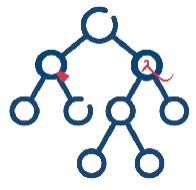
\includegraphics[height=1.0cm]{msca_logo.png}}%
    \end{center}

    \vspace{0.6cm}

    % Main title with Q logos on sides (with clickable links)
    \begin{center}
        \begin{minipage}{0.1\textwidth}
            \centering
            \href{https://quantlet.com}{
\includegraphics[height=1.1cm]{ql_logo.png}}
        \end{minipage}%
        \begin{minipage}{0.78\textwidth}
            \centering
            {\LARGE\bfseries\usebeamercolor[fg]{title}\inserttitle}

            \vspace{0.3cm}

            {\usebeamerfont{subtitle}\usebeamercolor[fg]{title}\insertsubtitle}
        \end{minipage}%
        \begin{minipage}{0.1\textwidth}
            \centering
            \href{https://quantinar.com}{
\includegraphics[height=1.1cm]{qr_logo.png}}
        \end{minipage}
    \end{center}

    \vspace{0.6cm}

    % Authors (left aligned)
    \hspace{0.5cm}{\usebeamerfont{author}\insertauthor}

    \vspace{0.3cm}

    % Institute/Affiliations (left aligned)
    \hspace{0.5cm}\begin{minipage}[t]{0.9\textwidth}
        \raggedright\small\insertinstitute
    \end{minipage}
}

%=============================================================================
% THEOREM ENVIRONMENTS
%=============================================================================
\theoremstyle{definition}
\setbeamertemplate{theorems}[numbered]
\ifdefined\tsalang
\newtheorem{defn}{Definiție}
\newtheorem{thm}{Teoremă}
\newtheorem{prop}{Propoziție}
\newtheorem{rmk}{Observație}
\else
\newtheorem{defn}{Definition}
\newtheorem{thm}{Theorem}
\newtheorem{prop}{Proposition}
\newtheorem{rmk}{Remark}
\fi

%=============================================================================
% CENTRED MINIPAGE (no extra vertical space)
%=============================================================================
\newenvironment{cminipage}[1]{%
    \par\noindent\hfill\begin{minipage}{#1}\ignorespaces
}{%
    \end{minipage}\hfill\null\par
}

%=============================================================================
% CUSTOM COMMANDS
%=============================================================================
\newcommand{\E}{\mathbb{E}}
\newcommand{\Var}{\text{Var}}
\newcommand{\Cov}{\text{Cov}}
\newcommand{\Corr}{\text{Corr}}
\newcommand{\R}{\mathbb{R}}
\newcommand{\N}{\mathbb{N}}
\newcommand{\Z}{\mathbb{Z}}
\newcommand{\B}{\mathbf{B}}
\newcommand{\imark}{\textcolor{MainBlue}{\textbullet}}
\newcommand{\RMSE}{\text{RMSE}}
\newcommand{\MAE}{\text{MAE}}
\newcommand{\MAPE}{\text{MAPE}}

% Boldface vector/matrix commands (VAR, VECM, state space; also used by the older TSA decks)
\newcommand{\bY}{\mathbf{Y}}
\newcommand{\bX}{\mathbf{X}}
\newcommand{\bA}{\mathbf{A}}
\newcommand{\bB}{\mathbf{B}}
\newcommand{\bepsilon}{\boldsymbol{\varepsilon}}
\newcommand{\bSigma}{\boldsymbol{\Sigma}}
\newcommand{\bPhi}{\boldsymbol{\Phi}}
\newcommand{\bGamma}{\boldsymbol{\Gamma}}
\newcommand{\bPi}{\boldsymbol{\Pi}}
\newcommand{\bc}{\mathbf{c}}
\newcommand{\balpha}{\boldsymbol{\alpha}}
\newcommand{\bbeta}{\boldsymbol{\beta}}
\newcommand{\bvarepsilon}{\boldsymbol{\varepsilon}}

% Legacy seminar marks (older TSA seminar decks)
\newcommand{\correct}{\textcolor{Forest}{\checkmark}}
\newcommand{\incorrect}{\textcolor{Crimson}{\texttimes}}
 se definește
%   \newcommand{\coursename}{Time Series Analysis}      (EN)
%   \newcommand{\coursename}{Serii de timp}       (RO)  și  \def\tsalang{ro}
% Fișierele .tex se află în EN/Courses, EN/Seminars, RO/Cursuri, RO/Seminarii (două niveluri sub rădăcină).
% Deck-urile sînt generate de latex/build_chapterN.py / build_seminarN.py (vezi latex/tsa_build.py).

\documentclass[9pt, aspectratio=169, t]{beamer}
\providecommand{\coursename}{Time Series Analysis}

% Ensure content fits on slides
\setbeamersize{text margin left=8mm, text margin right=8mm}
% Smaller institute font (title page)
\setbeamerfont{institute}{size=\footnotesize}

%=============================================================================
% THEME AND STYLE CONFIGURATION
%=============================================================================
\usetheme{default}
% Using default theme for clean header/footer control

% Color Palette (matching Redispatch PDF)
\definecolor{MainBlue}{RGB}{26, 58, 110}
\definecolor{AccentBlue}{RGB}{26, 58, 110}
\definecolor{IDAred}{RGB}{205, 0, 0}
\definecolor{DarkGray}{RGB}{51, 51, 51}
\definecolor{MediumGray}{RGB}{128, 128, 128}
\definecolor{LightGray}{RGB}{248, 248, 248}
\definecolor{VeryLightGray}{RGB}{235, 235, 235}
\definecolor{KeynoteGray}{RGB}{218, 218, 218}
\definecolor{SectionGray}{RGB}{120, 120, 120}
\definecolor{FooterGray}{RGB}{100, 100, 100}
\definecolor{Crimson}{RGB}{220, 53, 69}
\definecolor{Forest}{RGB}{46, 125, 50}
\definecolor{Amber}{RGB}{181, 133, 63}
\definecolor{Orange}{RGB}{230, 126, 34}
\definecolor{Purple}{RGB}{142, 68, 173}

% Gradient background (exact Keynote 315° gradient: white to RGB 218,218,218)
\setbeamertemplate{background}{%
    \begin{tikzpicture}[remember picture, overlay]
        \shade[shading=axis, shading angle=315,
        top color=white, bottom color=KeynoteGray]
        (current page.south west) rectangle (current page.north east);
    \end{tikzpicture}%
}
% Fallback solid color for compatibility
\setbeamercolor{background canvas}{bg=}

\setbeamercolor{palette primary}{bg=MainBlue, fg=white}
\setbeamercolor{palette secondary}{bg=MainBlue!85, fg=white}
\setbeamercolor{palette tertiary}{bg=MainBlue!70, fg=white}
\setbeamercolor{structure}{fg=MainBlue}
\setbeamercolor{title}{fg=IDAred}
\setbeamercolor{frametitle}{fg=IDAred, bg=}
\setbeamercolor{block title}{bg=MainBlue, fg=white}
\setbeamercolor{block body}{bg=VeryLightGray, fg=DarkGray}
\setbeamercolor{block title alerted}{bg=Crimson, fg=white}
\setbeamercolor{block body alerted}{bg=Crimson!8, fg=DarkGray}
\setbeamercolor{block title example}{bg=Forest, fg=white}
\setbeamercolor{block body example}{bg=Forest!8, fg=DarkGray}
\setbeamercolor{item}{fg=MainBlue}

% Footer colors (override Madrid theme blue)
\setbeamercolor{author in head/foot}{fg=FooterGray, bg=}
\setbeamercolor{title in head/foot}{fg=FooterGray, bg=}
\setbeamercolor{date in head/foot}{fg=FooterGray, bg=}
\setbeamercolor{section in head/foot}{fg=FooterGray, bg=}
\setbeamercolor{subsection in head/foot}{fg=FooterGray, bg=}

% Bullet styles (apply everywhere including blocks)
\setbeamertemplate{itemize item}{\color{MainBlue}$\boxdot$}
\setbeamertemplate{itemize subitem}{\color{MainBlue}$\blacktriangleright$}
\setbeamertemplate{itemize subsubitem}{\color{MainBlue}\tiny$\bullet$}
\setbeamertemplate{itemize/enumerate body begin}{\normalsize}
\setbeamertemplate{itemize/enumerate subbody begin}{\normalsize}

% Item spacing - compact style
\setlength{\leftmargini}{10pt}       % Level 1: minimal indent
\setlength{\leftmarginii}{10pt}      % Level 2: minimal additional indent
% Compact list spacing (zero extra space before/after lists in blocks)
\makeatletter
\def\@listi{\leftmargin\leftmargini \topsep 0pt \parsep 0pt \itemsep 0pt}
\def\@listii{\leftmargin\leftmarginii \topsep 0pt \parsep 0pt \itemsep 0pt}
\makeatother

\setbeamertemplate{navigation symbols}{}

%=============================================================================
% CUSTOM HEADLINE
%=============================================================================
\setbeamertemplate{headline}{%
    \vskip10pt%
    \hbox to \paperwidth{%
        \hskip0.5cm%
        {\small\color{FooterGray}\renewcommand{\hyperlink}[2]{##2}\insertsectionhead}%
        \hfill%
        \textcolor{FooterGray}{\small\insertframenumber}%
        \hskip0.5cm%
    }%
    \vskip4pt%
    {\color{FooterGray}\hrule height 0.4pt}%
}

%=============================================================================
% CUSTOM FOOTER
%=============================================================================
\usepackage{fontawesome5}

\setbeamertemplate{footline}{%
    {\color{FooterGray}\hrule height 0.4pt}%
    \vskip4pt%
    \hbox to \paperwidth{%
        \hskip0.5cm%
        \textcolor{FooterGray}{\small\coursename}%
        \hfill%
        \raisebox{-0.1em}{%
            \begin{tikzpicture}[x=0.08em, y=0.08em, line width=0.4pt]
                \draw[FooterGray] (0,3) -- (1,4) -- (2,3.5) -- (3,5) -- (4,4) -- (5,6) -- (6,5.5) -- (7,4) -- (8,5) -- (9,7) -- (10,6) -- (11,5) -- (12,6.5) -- (13,8) -- (14,7) -- (15,6) -- (16,7.5) -- (17,9) -- (18,8) -- (19,7) -- (20,8.5) -- (21,10) -- (22,9) -- (23,8) -- (24,9.5);
            \end{tikzpicture}%
        }%
        \hskip0.5cm%
    }%
    \vskip6pt%
}

%=============================================================================
% PACKAGES
%=============================================================================
\usepackage[utf8]{inputenc}
\DeclareUnicodeCharacter{03B1}{\ensuremath{\alpha}}
\usepackage[T1]{fontenc}
\usepackage{amsmath, amssymb, amsthm}
\usepackage{mathtools}
\usepackage{bm}
\usepackage{tikz}
\usetikzlibrary{arrows.meta, positioning, shapes, calc, decorations.pathreplacing, shadings}
\usepackage{booktabs}
\usepackage{multirow}
\usepackage{array}
\usepackage{graphicx}
\usepackage{animate}
\usepackage{hyperref}
\usepackage{colortbl}
\usepackage{listings}
\lstset{language=Python, basicstyle=\ttfamily\scriptsize, keywordstyle=\color{MainBlue}\bfseries,
  commentstyle=\color{Forest}, stringstyle=\color{Crimson}, breaklines=true,
  frame=none, backgroundcolor=\color{VeryLightGray}, xleftmargin=2mm}
\hypersetup{colorlinks=true, linkcolor=MainBlue, urlcolor=MainBlue}
\graphicspath{{../../logos/}{../../charts/}{../../photos/}}
\usepackage{xcolor}
\hfuzz=2pt  % Suppress tiny overfull warnings (<2pt)
\vfuzz=2pt  % Suppress tiny vertical overfull warnings (<2pt)
% \mathrm in the sans-serif family of the slides (beamer resets \mathrm to the serif family at \begin{document};
% this hook runs after beamer's, so WN, Var, RMSE, ... in formulas match the surrounding text)
% Bold vectors and matrices in the same sans-serif family: \mathbf{A} in sans bold (beamer's own \mathbf came out in
% medium weight), and the bold upright Greek capitals of \boldsymbol / \bm (\bSigma, \bPhi, \boldsymbol{\Theta}) in
% cmss bold: bm.sty fixes its "boldoperators" font when it is loaded (serif cmbx), before beamer switches the
% operators to cmss, so it is reset here.
\AtBeginDocument{%
  \SetMathAlphabet{\mathrm}{normal}{\encodingdefault}{\sfdefault}{\mddefault}{n}%
  \SetMathAlphabet{\mathrm}{bold}{\encodingdefault}{\sfdefault}{bx}{n}%
  \SetMathAlphabet{\mathbf}{normal}{\encodingdefault}{\sfdefault}{bx}{n}%
  \SetMathAlphabet{\mathbf}{bold}{\encodingdefault}{\sfdefault}{bx}{n}%
  \SetSymbolFont{boldoperators}{normal}{OT1}{cmss}{bx}{n}%
  \SetSymbolFont{boldoperators}{bold}{OT1}{cmss}{bx}{n}}

%=============================================================================
% QUANTLET COMMANDS
%   \quantlet{<displayed name>}{<url>}       (generic, compatible with the older TSA decks)
%   \tsaquantlet{Ch_05}{TSA_ch5_garch}       -> https://github.com/danpele/Time-Series-Analysis/tree/main/Quantlets/Ch_05/TSA_ch5_garch
%   \qlurl{<folder>} is defined per chapter by the generator (Quantlets/Ch_NN/<folder>)
%=============================================================================
\newcommand{\tsarepo}{https://github.com/danpele/Time-Series-Analysis}
\newcommand{\tsaqlbase}{https://github.com/danpele/Time-Series-Analysis/tree/main/Quantlets}
\newcommand{\quantlet}[2]{%
    \hfill\href{#2}{%
        \raisebox{-0.15em}{
\includegraphics[height=0.7em]{ql_logo.png}}%
        \textcolor{MainBlue}{\tiny\ #1}%
    }%
}
\newcommand{\tsaquantlet}[2]{\quantlet{\detokenize{#2}}{\tsaqlbase/#1/#2}}

%=============================================================================
% NOTEBOOKS (Google Colab)
%   \colaburl{notebooks/EN/chapter5_seminar_notebook.ipynb} -> the Colab link of a file in the TSA repo
%   \nb: the chapter notebook (each seminar deck redefines it with \renewcommand)
%=============================================================================
\newcommand{\colaburl}[1]{https://colab.research.google.com/github/danpele/Time-Series-Analysis/blob/main/#1}
\newcommand{\nb}{https://colab.research.google.com/github/danpele/Time-Series-Analysis/tree/main/notebooks/EN}
\newcommand{\nbname}{notebooks/EN}

%=============================================================================
% SLIDE HELPERS (used by the generators; the same as in MFM)
%=============================================================================
% local font size for list bodies (the preamble forces \normalsize)
\newcommand{\itemsize}[1]{\setbeamertemplate{itemize/enumerate body begin}{#1}\setbeamertemplate{itemize/enumerate subbody begin}{#1}}
\newcommand{\intitle}[1]{{\hypersetup{urlcolor=white}#1}}   % white links inside coloured title bars
\newcommand{\imgcap}[1]{{\scriptsize #1}\\[0.5mm]}          % caption under a photo
\newcommand{\imgcredit}[2]{{\tiny\color{FooterGray}\href{#1}{#2}}}   % image credit: source URL, author/licence
\newcommand{\aiprompt}[1]{{\ttfamily\color{MainBlue}#1}}     % a prompt to an AI assistant

%=============================================================================
% SEMINARS: student version by default; the instructor wrapper *_solutions.tex sets \solutionstrue
%=============================================================================
\makeatletter\@ifundefined{ifsolutions}{\expandafter\newif\csname ifsolutions\endcsname}{}\makeatother
\newcommand{\solonly}[1]{\ifsolutions #1\fi}
\newcommand{\propsub}{\ifsolutions\else\framesubtitle{\ifdefined\tsalang Rezolvarea se discută la seminar\else Solution discussed in class\fi}\fi}

%=============================================================================
% APPENDIX AND CHAPTER LINKS (latex/appendix_links.py writes the calls; it also re-declares these
% macros before \begin{document}, so the decks compile with or without this preamble block)
%=============================================================================
\providecommand{\tsaapplink}[3]{\hypertarget{#2}{}\hyperlink{#1}{\beamergotobutton{#3}}}
\providecommand{\tsaappback}[2]{\begin{tikzpicture}[remember picture,overlay]\node[anchor=south east] at ([xshift=-3mm,yshift=7mm]current page.south east){\hyperlink{#1}{\beamerreturnbutton{#2}}};\end{tikzpicture}}
\providecommand{\tsachlink}[2]{\href{#1}{#2}}
\providecommand{\tsachlinkt}[2]{\href{#1}{\usebeamercolor[fg]{frametitle}#2}}

%=============================================================================
% QUANTINAR COMMAND: link către un curs Quantinar (subiecte avansate)
%=============================================================================
\newcommand{\quantinar}[2]{%
    \href{#2}{%
        \raisebox{-0.15em}{
\includegraphics[height=0.8em]{qr_logo.png}}%
        \textcolor{MainBlue}{\scriptsize\ #1}%
    }%
}

%=============================================================================
% CUSTOM TITLE PAGE
%=============================================================================
\defbeamertemplate*{title page}{hybrid}[1][]
{
    \vspace{0.2cm}
    % Logos row - top header (with clickable links)
    \begin{center}
        \href{https://www.ase.ro}{
\includegraphics[height=1.0cm]{ase_logo.png}}\hspace{0.3cm}%
        \href{https://theida.net}{
\includegraphics[height=1.0cm]{ida_logo.png}}\hspace{0.3cm}%
        \href{https://blockchain-research-center.com}{
\includegraphics[height=1.0cm]{brc_logo.png}}\hspace{0.3cm}%
        \href{https://www.ai4efin.ase.ro}{
\includegraphics[height=1.0cm]{ai4efin_logo.png}}\hspace{0.3cm}%
        \href{https://ipe.ro/new}{
\includegraphics[height=1.0cm]{acad_logo.png}}\hspace{0.3cm}%
        \href{https://www.digital-finance-msca.com}{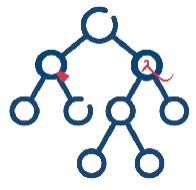
\includegraphics[height=1.0cm]{msca_logo.png}}%
    \end{center}

    \vspace{0.6cm}

    % Main title with Q logos on sides (with clickable links)
    \begin{center}
        \begin{minipage}{0.1\textwidth}
            \centering
            \href{https://quantlet.com}{
\includegraphics[height=1.1cm]{ql_logo.png}}
        \end{minipage}%
        \begin{minipage}{0.78\textwidth}
            \centering
            {\LARGE\bfseries\usebeamercolor[fg]{title}\inserttitle}

            \vspace{0.3cm}

            {\usebeamerfont{subtitle}\usebeamercolor[fg]{title}\insertsubtitle}
        \end{minipage}%
        \begin{minipage}{0.1\textwidth}
            \centering
            \href{https://quantinar.com}{
\includegraphics[height=1.1cm]{qr_logo.png}}
        \end{minipage}
    \end{center}

    \vspace{0.6cm}

    % Authors (left aligned)
    \hspace{0.5cm}{\usebeamerfont{author}\insertauthor}

    \vspace{0.3cm}

    % Institute/Affiliations (left aligned)
    \hspace{0.5cm}\begin{minipage}[t]{0.9\textwidth}
        \raggedright\small\insertinstitute
    \end{minipage}
}

%=============================================================================
% THEOREM ENVIRONMENTS
%=============================================================================
\theoremstyle{definition}
\setbeamertemplate{theorems}[numbered]
\ifdefined\tsalang
\newtheorem{defn}{Definiție}
\newtheorem{thm}{Teoremă}
\newtheorem{prop}{Propoziție}
\newtheorem{rmk}{Observație}
\else
\newtheorem{defn}{Definition}
\newtheorem{thm}{Theorem}
\newtheorem{prop}{Proposition}
\newtheorem{rmk}{Remark}
\fi

%=============================================================================
% CENTRED MINIPAGE (no extra vertical space)
%=============================================================================
\newenvironment{cminipage}[1]{%
    \par\noindent\hfill\begin{minipage}{#1}\ignorespaces
}{%
    \end{minipage}\hfill\null\par
}

%=============================================================================
% CUSTOM COMMANDS
%=============================================================================
\newcommand{\E}{\mathbb{E}}
\newcommand{\Var}{\text{Var}}
\newcommand{\Cov}{\text{Cov}}
\newcommand{\Corr}{\text{Corr}}
\newcommand{\R}{\mathbb{R}}
\newcommand{\N}{\mathbb{N}}
\newcommand{\Z}{\mathbb{Z}}
\newcommand{\B}{\mathbf{B}}
\newcommand{\imark}{\textcolor{MainBlue}{\textbullet}}
\newcommand{\RMSE}{\text{RMSE}}
\newcommand{\MAE}{\text{MAE}}
\newcommand{\MAPE}{\text{MAPE}}

% Boldface vector/matrix commands (VAR, VECM, state space; also used by the older TSA decks)
\newcommand{\bY}{\mathbf{Y}}
\newcommand{\bX}{\mathbf{X}}
\newcommand{\bA}{\mathbf{A}}
\newcommand{\bB}{\mathbf{B}}
\newcommand{\bepsilon}{\boldsymbol{\varepsilon}}
\newcommand{\bSigma}{\boldsymbol{\Sigma}}
\newcommand{\bPhi}{\boldsymbol{\Phi}}
\newcommand{\bGamma}{\boldsymbol{\Gamma}}
\newcommand{\bPi}{\boldsymbol{\Pi}}
\newcommand{\bc}{\mathbf{c}}
\newcommand{\balpha}{\boldsymbol{\alpha}}
\newcommand{\bbeta}{\boldsymbol{\beta}}
\newcommand{\bvarepsilon}{\boldsymbol{\varepsilon}}

% Legacy seminar marks (older TSA seminar decks)
\newcommand{\correct}{\textcolor{Forest}{\checkmark}}
\newcommand{\incorrect}{\textcolor{Crimson}{\texttimes}}
 se definește
%   \newcommand{\coursename}{Time Series Analysis}      (EN)
%   \newcommand{\coursename}{Serii de timp}       (RO)  și  \def\tsalang{ro}
% Fișierele .tex se află în EN/Courses, EN/Seminars, RO/Cursuri, RO/Seminarii (două niveluri sub rădăcină).
% Deck-urile sînt generate de latex/build_chapterN.py / build_seminarN.py (vezi latex/tsa_build.py).

\documentclass[9pt, aspectratio=169, t]{beamer}
\providecommand{\coursename}{Time Series Analysis}

% Ensure content fits on slides
\setbeamersize{text margin left=8mm, text margin right=8mm}
% Smaller institute font (title page)
\setbeamerfont{institute}{size=\footnotesize}

%=============================================================================
% THEME AND STYLE CONFIGURATION
%=============================================================================
\usetheme{default}
% Using default theme for clean header/footer control

% Color Palette (matching Redispatch PDF)
\definecolor{MainBlue}{RGB}{26, 58, 110}
\definecolor{AccentBlue}{RGB}{26, 58, 110}
\definecolor{IDAred}{RGB}{205, 0, 0}
\definecolor{DarkGray}{RGB}{51, 51, 51}
\definecolor{MediumGray}{RGB}{128, 128, 128}
\definecolor{LightGray}{RGB}{248, 248, 248}
\definecolor{VeryLightGray}{RGB}{235, 235, 235}
\definecolor{KeynoteGray}{RGB}{218, 218, 218}
\definecolor{SectionGray}{RGB}{120, 120, 120}
\definecolor{FooterGray}{RGB}{100, 100, 100}
\definecolor{Crimson}{RGB}{220, 53, 69}
\definecolor{Forest}{RGB}{46, 125, 50}
\definecolor{Amber}{RGB}{181, 133, 63}
\definecolor{Orange}{RGB}{230, 126, 34}
\definecolor{Purple}{RGB}{142, 68, 173}

% Gradient background (exact Keynote 315° gradient: white to RGB 218,218,218)
\setbeamertemplate{background}{%
    \begin{tikzpicture}[remember picture, overlay]
        \shade[shading=axis, shading angle=315,
        top color=white, bottom color=KeynoteGray]
        (current page.south west) rectangle (current page.north east);
    \end{tikzpicture}%
}
% Fallback solid color for compatibility
\setbeamercolor{background canvas}{bg=}

\setbeamercolor{palette primary}{bg=MainBlue, fg=white}
\setbeamercolor{palette secondary}{bg=MainBlue!85, fg=white}
\setbeamercolor{palette tertiary}{bg=MainBlue!70, fg=white}
\setbeamercolor{structure}{fg=MainBlue}
\setbeamercolor{title}{fg=IDAred}
\setbeamercolor{frametitle}{fg=IDAred, bg=}
\setbeamercolor{block title}{bg=MainBlue, fg=white}
\setbeamercolor{block body}{bg=VeryLightGray, fg=DarkGray}
\setbeamercolor{block title alerted}{bg=Crimson, fg=white}
\setbeamercolor{block body alerted}{bg=Crimson!8, fg=DarkGray}
\setbeamercolor{block title example}{bg=Forest, fg=white}
\setbeamercolor{block body example}{bg=Forest!8, fg=DarkGray}
\setbeamercolor{item}{fg=MainBlue}

% Footer colors (override Madrid theme blue)
\setbeamercolor{author in head/foot}{fg=FooterGray, bg=}
\setbeamercolor{title in head/foot}{fg=FooterGray, bg=}
\setbeamercolor{date in head/foot}{fg=FooterGray, bg=}
\setbeamercolor{section in head/foot}{fg=FooterGray, bg=}
\setbeamercolor{subsection in head/foot}{fg=FooterGray, bg=}

% Bullet styles (apply everywhere including blocks)
\setbeamertemplate{itemize item}{\color{MainBlue}$\boxdot$}
\setbeamertemplate{itemize subitem}{\color{MainBlue}$\blacktriangleright$}
\setbeamertemplate{itemize subsubitem}{\color{MainBlue}\tiny$\bullet$}
\setbeamertemplate{itemize/enumerate body begin}{\normalsize}
\setbeamertemplate{itemize/enumerate subbody begin}{\normalsize}

% Item spacing - compact style
\setlength{\leftmargini}{10pt}       % Level 1: minimal indent
\setlength{\leftmarginii}{10pt}      % Level 2: minimal additional indent
% Compact list spacing (zero extra space before/after lists in blocks)
\makeatletter
\def\@listi{\leftmargin\leftmargini \topsep 0pt \parsep 0pt \itemsep 0pt}
\def\@listii{\leftmargin\leftmarginii \topsep 0pt \parsep 0pt \itemsep 0pt}
\makeatother

\setbeamertemplate{navigation symbols}{}

%=============================================================================
% CUSTOM HEADLINE
%=============================================================================
\setbeamertemplate{headline}{%
    \vskip10pt%
    \hbox to \paperwidth{%
        \hskip0.5cm%
        {\small\color{FooterGray}\renewcommand{\hyperlink}[2]{##2}\insertsectionhead}%
        \hfill%
        \textcolor{FooterGray}{\small\insertframenumber}%
        \hskip0.5cm%
    }%
    \vskip4pt%
    {\color{FooterGray}\hrule height 0.4pt}%
}

%=============================================================================
% CUSTOM FOOTER
%=============================================================================
\usepackage{fontawesome5}

\setbeamertemplate{footline}{%
    {\color{FooterGray}\hrule height 0.4pt}%
    \vskip4pt%
    \hbox to \paperwidth{%
        \hskip0.5cm%
        \textcolor{FooterGray}{\small\coursename}%
        \hfill%
        \raisebox{-0.1em}{%
            \begin{tikzpicture}[x=0.08em, y=0.08em, line width=0.4pt]
                \draw[FooterGray] (0,3) -- (1,4) -- (2,3.5) -- (3,5) -- (4,4) -- (5,6) -- (6,5.5) -- (7,4) -- (8,5) -- (9,7) -- (10,6) -- (11,5) -- (12,6.5) -- (13,8) -- (14,7) -- (15,6) -- (16,7.5) -- (17,9) -- (18,8) -- (19,7) -- (20,8.5) -- (21,10) -- (22,9) -- (23,8) -- (24,9.5);
            \end{tikzpicture}%
        }%
        \hskip0.5cm%
    }%
    \vskip6pt%
}

%=============================================================================
% PACKAGES
%=============================================================================
\usepackage[utf8]{inputenc}
\DeclareUnicodeCharacter{03B1}{\ensuremath{\alpha}}
\usepackage[T1]{fontenc}
\usepackage{amsmath, amssymb, amsthm}
\usepackage{mathtools}
\usepackage{bm}
\usepackage{tikz}
\usetikzlibrary{arrows.meta, positioning, shapes, calc, decorations.pathreplacing, shadings}
\usepackage{booktabs}
\usepackage{multirow}
\usepackage{array}
\usepackage{graphicx}
\usepackage{animate}
\usepackage{hyperref}
\usepackage{colortbl}
\usepackage{listings}
\lstset{language=Python, basicstyle=\ttfamily\scriptsize, keywordstyle=\color{MainBlue}\bfseries,
  commentstyle=\color{Forest}, stringstyle=\color{Crimson}, breaklines=true,
  frame=none, backgroundcolor=\color{VeryLightGray}, xleftmargin=2mm}
\hypersetup{colorlinks=true, linkcolor=MainBlue, urlcolor=MainBlue}
\graphicspath{{../../logos/}{../../charts/}{../../photos/}}
\usepackage{xcolor}
\hfuzz=2pt  % Suppress tiny overfull warnings (<2pt)
\vfuzz=2pt  % Suppress tiny vertical overfull warnings (<2pt)
% \mathrm in the sans-serif family of the slides (beamer resets \mathrm to the serif family at \begin{document};
% this hook runs after beamer's, so WN, Var, RMSE, ... in formulas match the surrounding text)
% Bold vectors and matrices in the same sans-serif family: \mathbf{A} in sans bold (beamer's own \mathbf came out in
% medium weight), and the bold upright Greek capitals of \boldsymbol / \bm (\bSigma, \bPhi, \boldsymbol{\Theta}) in
% cmss bold: bm.sty fixes its "boldoperators" font when it is loaded (serif cmbx), before beamer switches the
% operators to cmss, so it is reset here.
\AtBeginDocument{%
  \SetMathAlphabet{\mathrm}{normal}{\encodingdefault}{\sfdefault}{\mddefault}{n}%
  \SetMathAlphabet{\mathrm}{bold}{\encodingdefault}{\sfdefault}{bx}{n}%
  \SetMathAlphabet{\mathbf}{normal}{\encodingdefault}{\sfdefault}{bx}{n}%
  \SetMathAlphabet{\mathbf}{bold}{\encodingdefault}{\sfdefault}{bx}{n}%
  \SetSymbolFont{boldoperators}{normal}{OT1}{cmss}{bx}{n}%
  \SetSymbolFont{boldoperators}{bold}{OT1}{cmss}{bx}{n}}

%=============================================================================
% QUANTLET COMMANDS
%   \quantlet{<displayed name>}{<url>}       (generic, compatible with the older TSA decks)
%   \tsaquantlet{Ch_05}{TSA_ch5_garch}       -> https://github.com/danpele/Time-Series-Analysis/tree/main/Quantlets/Ch_05/TSA_ch5_garch
%   \qlurl{<folder>} is defined per chapter by the generator (Quantlets/Ch_NN/<folder>)
%=============================================================================
\newcommand{\tsarepo}{https://github.com/danpele/Time-Series-Analysis}
\newcommand{\tsaqlbase}{https://github.com/danpele/Time-Series-Analysis/tree/main/Quantlets}
\newcommand{\quantlet}[2]{%
    \hfill\href{#2}{%
        \raisebox{-0.15em}{
\includegraphics[height=0.7em]{ql_logo.png}}%
        \textcolor{MainBlue}{\tiny\ #1}%
    }%
}
\newcommand{\tsaquantlet}[2]{\quantlet{\detokenize{#2}}{\tsaqlbase/#1/#2}}

%=============================================================================
% NOTEBOOKS (Google Colab)
%   \colaburl{notebooks/EN/chapter5_seminar_notebook.ipynb} -> the Colab link of a file in the TSA repo
%   \nb: the chapter notebook (each seminar deck redefines it with \renewcommand)
%=============================================================================
\newcommand{\colaburl}[1]{https://colab.research.google.com/github/danpele/Time-Series-Analysis/blob/main/#1}
\newcommand{\nb}{https://colab.research.google.com/github/danpele/Time-Series-Analysis/tree/main/notebooks/EN}
\newcommand{\nbname}{notebooks/EN}

%=============================================================================
% SLIDE HELPERS (used by the generators; the same as in MFM)
%=============================================================================
% local font size for list bodies (the preamble forces \normalsize)
\newcommand{\itemsize}[1]{\setbeamertemplate{itemize/enumerate body begin}{#1}\setbeamertemplate{itemize/enumerate subbody begin}{#1}}
\newcommand{\intitle}[1]{{\hypersetup{urlcolor=white}#1}}   % white links inside coloured title bars
\newcommand{\imgcap}[1]{{\scriptsize #1}\\[0.5mm]}          % caption under a photo
\newcommand{\imgcredit}[2]{{\tiny\color{FooterGray}\href{#1}{#2}}}   % image credit: source URL, author/licence
\newcommand{\aiprompt}[1]{{\ttfamily\color{MainBlue}#1}}     % a prompt to an AI assistant

%=============================================================================
% SEMINARS: student version by default; the instructor wrapper *_solutions.tex sets \solutionstrue
%=============================================================================
\makeatletter\@ifundefined{ifsolutions}{\expandafter\newif\csname ifsolutions\endcsname}{}\makeatother
\newcommand{\solonly}[1]{\ifsolutions #1\fi}
\newcommand{\propsub}{\ifsolutions\else\framesubtitle{\ifdefined\tsalang Rezolvarea se discută la seminar\else Solution discussed in class\fi}\fi}

%=============================================================================
% APPENDIX AND CHAPTER LINKS (latex/appendix_links.py writes the calls; it also re-declares these
% macros before \begin{document}, so the decks compile with or without this preamble block)
%=============================================================================
\providecommand{\tsaapplink}[3]{\hypertarget{#2}{}\hyperlink{#1}{\beamergotobutton{#3}}}
\providecommand{\tsaappback}[2]{\begin{tikzpicture}[remember picture,overlay]\node[anchor=south east] at ([xshift=-3mm,yshift=7mm]current page.south east){\hyperlink{#1}{\beamerreturnbutton{#2}}};\end{tikzpicture}}
\providecommand{\tsachlink}[2]{\href{#1}{#2}}
\providecommand{\tsachlinkt}[2]{\href{#1}{\usebeamercolor[fg]{frametitle}#2}}

%=============================================================================
% QUANTINAR COMMAND: link către un curs Quantinar (subiecte avansate)
%=============================================================================
\newcommand{\quantinar}[2]{%
    \href{#2}{%
        \raisebox{-0.15em}{
\includegraphics[height=0.8em]{qr_logo.png}}%
        \textcolor{MainBlue}{\scriptsize\ #1}%
    }%
}

%=============================================================================
% CUSTOM TITLE PAGE
%=============================================================================
\defbeamertemplate*{title page}{hybrid}[1][]
{
    \vspace{0.2cm}
    % Logos row - top header (with clickable links)
    \begin{center}
        \href{https://www.ase.ro}{
\includegraphics[height=1.0cm]{ase_logo.png}}\hspace{0.3cm}%
        \href{https://theida.net}{
\includegraphics[height=1.0cm]{ida_logo.png}}\hspace{0.3cm}%
        \href{https://blockchain-research-center.com}{
\includegraphics[height=1.0cm]{brc_logo.png}}\hspace{0.3cm}%
        \href{https://www.ai4efin.ase.ro}{
\includegraphics[height=1.0cm]{ai4efin_logo.png}}\hspace{0.3cm}%
        \href{https://ipe.ro/new}{
\includegraphics[height=1.0cm]{acad_logo.png}}\hspace{0.3cm}%
        \href{https://www.digital-finance-msca.com}{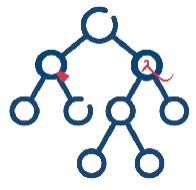
\includegraphics[height=1.0cm]{msca_logo.png}}%
    \end{center}

    \vspace{0.6cm}

    % Main title with Q logos on sides (with clickable links)
    \begin{center}
        \begin{minipage}{0.1\textwidth}
            \centering
            \href{https://quantlet.com}{
\includegraphics[height=1.1cm]{ql_logo.png}}
        \end{minipage}%
        \begin{minipage}{0.78\textwidth}
            \centering
            {\LARGE\bfseries\usebeamercolor[fg]{title}\inserttitle}

            \vspace{0.3cm}

            {\usebeamerfont{subtitle}\usebeamercolor[fg]{title}\insertsubtitle}
        \end{minipage}%
        \begin{minipage}{0.1\textwidth}
            \centering
            \href{https://quantinar.com}{
\includegraphics[height=1.1cm]{qr_logo.png}}
        \end{minipage}
    \end{center}

    \vspace{0.6cm}

    % Authors (left aligned)
    \hspace{0.5cm}{\usebeamerfont{author}\insertauthor}

    \vspace{0.3cm}

    % Institute/Affiliations (left aligned)
    \hspace{0.5cm}\begin{minipage}[t]{0.9\textwidth}
        \raggedright\small\insertinstitute
    \end{minipage}
}

%=============================================================================
% THEOREM ENVIRONMENTS
%=============================================================================
\theoremstyle{definition}
\setbeamertemplate{theorems}[numbered]
\ifdefined\tsalang
\newtheorem{defn}{Definiție}
\newtheorem{thm}{Teoremă}
\newtheorem{prop}{Propoziție}
\newtheorem{rmk}{Observație}
\else
\newtheorem{defn}{Definition}
\newtheorem{thm}{Theorem}
\newtheorem{prop}{Proposition}
\newtheorem{rmk}{Remark}
\fi

%=============================================================================
% CENTRED MINIPAGE (no extra vertical space)
%=============================================================================
\newenvironment{cminipage}[1]{%
    \par\noindent\hfill\begin{minipage}{#1}\ignorespaces
}{%
    \end{minipage}\hfill\null\par
}

%=============================================================================
% CUSTOM COMMANDS
%=============================================================================
\newcommand{\E}{\mathbb{E}}
\newcommand{\Var}{\text{Var}}
\newcommand{\Cov}{\text{Cov}}
\newcommand{\Corr}{\text{Corr}}
\newcommand{\R}{\mathbb{R}}
\newcommand{\N}{\mathbb{N}}
\newcommand{\Z}{\mathbb{Z}}
\newcommand{\B}{\mathbf{B}}
\newcommand{\imark}{\textcolor{MainBlue}{\textbullet}}
\newcommand{\RMSE}{\text{RMSE}}
\newcommand{\MAE}{\text{MAE}}
\newcommand{\MAPE}{\text{MAPE}}

% Boldface vector/matrix commands (VAR, VECM, state space; also used by the older TSA decks)
\newcommand{\bY}{\mathbf{Y}}
\newcommand{\bX}{\mathbf{X}}
\newcommand{\bA}{\mathbf{A}}
\newcommand{\bB}{\mathbf{B}}
\newcommand{\bepsilon}{\boldsymbol{\varepsilon}}
\newcommand{\bSigma}{\boldsymbol{\Sigma}}
\newcommand{\bPhi}{\boldsymbol{\Phi}}
\newcommand{\bGamma}{\boldsymbol{\Gamma}}
\newcommand{\bPi}{\boldsymbol{\Pi}}
\newcommand{\bc}{\mathbf{c}}
\newcommand{\balpha}{\boldsymbol{\alpha}}
\newcommand{\bbeta}{\boldsymbol{\beta}}
\newcommand{\bvarepsilon}{\boldsymbol{\varepsilon}}

% Legacy seminar marks (older TSA seminar decks)
\newcommand{\correct}{\textcolor{Forest}{\checkmark}}
\newcommand{\incorrect}{\textcolor{Crimson}{\texttimes}}


\newcommand{\qlurl}[1]{https://github.com/danpele/Time-Series-Analysis/tree/main/Quantlets/Ch_10/#1}
\renewcommand{\nb}{\colaburl{notebooks/EN/chapter10_seminar_notebook.ipynb}}
\renewcommand{\nbname}{chapter10\_seminar\_notebook.ipynb}
% left column: full width in the student version, narrower next to the solution
\newcommand{\taskw}{\ifsolutions 0.47\textwidth\else 0.96\textwidth\fi}
\newcommand{\solw}{\ifsolutions 0.49\textwidth\else 0pt\fi}

% Clickable citations (DOIs verified via Crossref)
\newcommand{\refHP}{\href{https://doi.org/10.1007/978-3-031-13584-2}{Huang și Petukhina (2022)}}
\newcommand{\refDK}{\href{https://doi.org/10.1093/acprof:oso/9780199641178.001.0001}{Durbin și Koopman (2012)}}
\newcommand{\refHarvey}{\href{https://doi.org/10.1017/CBO9781107049994}{Harvey (1989)}}
\newcommand{\refHamilton}{\href{https://doi.org/10.2307/j.ctv14jx6sm}{Hamilton (1994)}}
\newcommand{\refKN}{\href{https://doi.org/10.7551/mitpress/6444.001.0001}{Kim și Nelson (1999)}}
\newcommand{\refSS}{\href{https://doi.org/10.1007/978-3-319-52452-8}{Shumway și Stoffer (2017)}}
\newcommand{\refKalman}{\href{https://doi.org/10.1115/1.3662552}{Kalman (1960)}}
\newcommand{\refRTS}{\href{https://doi.org/10.2514/3.3166}{Rauch, Tung și Striebel (1965)}}
\newcommand{\refMuth}{\href{https://doi.org/10.1080/01621459.1960.10482064}{Muth (1960)}}
\newcommand{\refHKOS}{\href{https://doi.org/10.1007/978-3-540-71918-2}{Hyndman et al.\ (2008)}}
\newcommand{\refHJ}{\href{https://doi.org/10.1002/jae.3950080302}{Harvey și Jaeger (1993)}}
\newcommand{\refHPf}{\href{https://doi.org/10.2307/2953682}{Hodrick și Prescott (1997)}}
\newcommand{\refHamHP}{\href{https://doi.org/10.1162/rest\_a\_00706}{Hamilton (2018)}}
\newcommand{\refSW}{\href{https://doi.org/10.1086/654119}{Stock și Watson (1989)}}
\newcommand{\refGRS}{\href{https://doi.org/10.1016/j.jmoneco.2008.05.010}{Giannone, Reichlin și Small (2008)}}
\newcommand{\refHamMS}{\href{https://doi.org/10.2307/1912559}{Hamilton (1989)}}
\newcommand{\refHamEM}{\href{https://doi.org/10.1016/0304-4076(90)90093-9}{Hamilton (1990)}}
\newcommand{\refKim}{\href{https://doi.org/10.1016/0304-4076(94)90036-1}{Kim (1994)}}
\newcommand{\refCP}{\href{https://doi.org/10.1198/073500107000000296}{Chauvet și Piger (2008)}}
\newcommand{\refHSus}{\href{https://doi.org/10.1016/0304-4076(94)90067-1}{Hamilton și Susmel (1994)}}
\newcommand{\refLL}{\href{https://doi.org/10.1080/07350015.1990.10509794}{Lamoureux și Lastrapes (1990)}}
\newcommand{\refDI}{\href{https://doi.org/10.1016/S0304-4076(01)00073-2}{Diebold și Inoue (2001)}}

\title[Serii de timp]{Serii de timp}
\subtitle{Seminarul 10: Modele în spațiul stărilor, filtrul Kalman și modele Markov switching\ifsolutions\ (versiunea profesorului)\fi}
\author[D.T. Pele]{Daniel Traian PELE}
\institute{Academia de Studii Economice din București\\
IDA Institute Digital Assets\\
Blockchain Research Center\\
AI4EFin Artificial Intelligence for Energy Finance\\
Academia Română, Institutul de Prognoză Economică\\
MSCA Digital Finance}
\date{}

%=============================================================================
\providecommand{\tsaapplink}[3]{\hypertarget{#2}{}\hyperlink{#1}{\beamergotobutton{#3}}}  % APPLINKS-MACROS
\providecommand{\tsaappback}[2]{\begin{tikzpicture}[remember picture,overlay]\node[anchor=south east] at ([xshift=-3mm,yshift=7mm]current page.south east){\hyperlink{#1}{\beamerreturnbutton{#2}}};\end{tikzpicture}}  % APPLINKS-MACROS
\providecommand{\tsachlink}[2]{\href{#1}{#2}}  % APPLINKS-MACROS
\providecommand{\tsachlinkt}[2]{\href{#1}{\usebeamercolor[fg]{frametitle}#2}}  % APPLINKS-MACROS
\begin{document}
%=============================================================================

{
\setbeamertemplate{headline}{}
\setbeamertemplate{footline}{}
\begin{frame}[noframenumbering]
    \titlepage
\end{frame}
}
% BEGIN-ACRONYMS (generat de latex/acronyms.py; nu editati manual)
\begin{frame}{Acronime folosite în acest material}
\setbeamertemplate{itemize/enumerate body begin}{\tiny}
\begin{columns}[T]
\begin{column}{0.49\textwidth}
\begin{itemize}\setlength{\itemsep}{0pt}
    \item \textbf{AI}: Artificial Intelligence (inteligență artificială)
    \item \textbf{AR}: AutoRegressive (model); in event studies: Abnormal Return (model autoregresiv; în studiile de eveniment: randament anormal)
    \item \textbf{BET}: Bucharest Exchange Trading (index) — indicele de referință al Bursei de Valori București
    \item \textbf{BIC}: Bayesian Information Criterion (criteriul informațional bayesian (Schwarz))
    \item \textbf{CBO}: Congressional Budget Office (oficiul pentru buget al Congresului SUA)
    \item \textbf{EODHD}: EOD Historical Data (market-data provider) — furnizor de date de piață
    \item \textbf{FRED}: Federal Reserve Economic Data (baza de date economice a Rezervei Federale din St. Louis)
    \item \textbf{GARCH}: Generalised AutoRegressive Conditional Heteroskedasticity (heteroscedasticitate condiționată autoregresivă generalizată)
    \item \textbf{GDPC1}: Real Gross Domestic Product, chained dollars (FRED series code) — codul FRED al PIB-ului real al SUA
    \item \textbf{GDPPOT}: Real Potential Gross Domestic Product (FRED series code) — codul FRED al PIB-ului potențial al SUA
    \item \textbf{HP}: Hodrick–Prescott (filter) — filtrul Hodrick–Prescott
    \item \textbf{IAPC}: Indicele armonizat al prețurilor de consum
    \item \textbf{INDPRO}: Industrial Production Index (FRED series code) — codul FRED al indicelui producției industriale din SUA
\end{itemize}
\end{column}
\begin{column}{0.49\textwidth}
\begin{itemize}\setlength{\itemsep}{0pt}
    \item \textbf{NBER}: National Bureau of Economic Research (biroul național de cercetare economică al SUA, care datează recesiunile)
    \item \textbf{OLS}: Ordinary Least Squares (metoda celor mai mici pătrate)
    \item \textbf{PIB}: Produsul intern brut
    \item \textbf{SD}: Standard Deviation (abaterea standard)
    \item \textbf{SE}: Standard Error (eroare standard)
    \item \textbf{SES}: Simple Exponential Smoothing (netezire exponențială simplă)
    \item \textbf{SUA}: Statele Unite ale Americii
    \item \textbf{TVA}: Taxa pe valoarea adăugată
    \item \textbf{UC}: Unobserved Components (model) — model cu componente neobservate
    \item \textbf{USREC}: US Recession indicator (FRED series code) — codul FRED al indicatorului de recesiune NBER
\end{itemize}
\end{column}
\end{columns}
\end{frame}
% END-ACRONYMS

\begin{frame}{Întrebarea de azi și traseul}
\itemsize{\small}
\begin{itemize}
    \item \textbf{Întrebarea}: cum estimăm o mărime pe care nu o observăm niciodată (un nivel, un trend, un regim) din date zgomotoase, perioadă cu perioadă?
    \begin{itemize}
        \item seminarul are loc \textbf{înaintea} Cursului 10: secțiunea „Noțiuni necesare azi” dă toate definițiile folosite în cerințe
    \end{itemize}
    \item Traseul
    \begin{itemize}
        \item Partea A: filtrul Kalman de mînă; netezirea exponențială ca stare de echilibru; forme în spațiul stărilor; durate; filtrul Hamilton
        \item Partea B: inflația din România; deviația PIB a SUA; producția industrială din SUA și recesiunile; regimurile de volatilitate ale BET
        \item Partea C: regimurile inflației din România din 1996; un răspuns AI de verificat
    \end{itemize}
    \item Notebook-ul de azi: \href{\nb}{deschideți notebook-ul seminarului în Google Colab}; fiecare cerință indică secțiunea din notebook
\end{itemize}
\end{frame}

\begin{frame}{Harta exercițiilor}
\itemsize{\small}
\begin{center}
\footnotesize
\begin{tabular}{>{\raggedright\arraybackslash}p{1.1cm}>{\raggedright\arraybackslash}p{7.5cm}>{\raggedright\arraybackslash}p{1.9cm}>{\raggedright\arraybackslash}p{1.4cm}}
\toprule
\textbf{Cerința} & \textbf{Întrebarea} & \textbf{Tipul} & \textbf{Model} \\
\midrule
A1, A2 & filtrul Kalman al unui model local level pentru trei perioade; o valoare lipsă & Rezolvat, Propus & A1 \\
A3, A4 & starea de echilibru și netezirea exponențială; forme în spațiul stărilor și prognoze & Rezolvat, Propus & A3 \\
A5, A6 & duratele regimurilor; un pas al filtrului Hamilton & Rezolvat, Propus & A5 \\
B1, B2 & inflația de fond din România; deviația PIB a SUA & Rezolvat, Propus & B1 \\
B3, B4 & recesiunile în producția industrială din SUA; regimurile de volatilitate ale BET & Rezolvat, Propus & B3 \\
C1, C2 & regimurile inflației din România; ce este greșit într-un răspuns AI? & Propus & B3, A1--A6 \\
\bottomrule
\end{tabular}
\end{center}
\begin{itemize}
    \item \textbf{[Rezolvat]}: rezolvarea completă în slide-uri și în notebook, un model de urmat; \textbf{[Propus]}: îl rezolvați dumneavoastră, după model
\end{itemize}
\end{frame}

\begin{frame}{Datele folosite}
\itemsize{\small}
\begin{center}
\footnotesize
\begin{tabular}{llll}
\toprule
\textbf{Seria} & \textbf{Sursa} & \textbf{Frecvența} & \textbf{Perioada} \\
\midrule
IAPC, România & Eurostat (prc\_hicp\_minr) & lunar, 2015 = 100 & 1996--2026 \\
PIB real și PIB potențial, SUA & FRED (GDPC1, GDPPOT) & trimestrial & 1947--2026 \\
producția industrială, SUA & FRED (INDPRO) & lunar & 1960--2019 \\
indicatorul de recesiune NBER & FRED (USREC) & lunar & 1960--2019 \\
BET, S\&P 500 & EODHD & săptămînal, din închideri zilnice & 2000--2026 \\
\bottomrule
\end{tabular}
\end{center}
\begin{itemize}
    \item Inflația lunară: $100\Delta\ln P_t$, ajustată sezonier (SA) prin eliminarea mediilor lunare (\tsachlink{https://danpele.github.io/Time-Series-Analysis/RO/Cursuri/capitol4_sezonalitate_prognoza.pdf}{Capitolul 4}); deviația PIB a CBO: $100(\mathrm{PIB}_t/\mathrm{GDPPOT}_t - 1)$
    \item În notebook: \texttt{kalman\_by\_hand}, \texttt{local\_level\_ml}, \texttt{uc\_fit}, \texttt{hamilton\_filter}, \texttt{MarkovRegression}; nu este nevoie de cont sau de cheie
\end{itemize}
\end{frame}


%=============================================================================
\section{Noțiuni necesare azi}
%=============================================================================

\begin{frame}{Noțiuni necesare azi (1/4): forma în spațiul stărilor}
\itemsize{\small}
\begin{itemize}
    \item \textbf{Forma în spațiul stărilor}: $y_t = Z\alpha_t + \varepsilon_t$ (măsurare), $\alpha_{t+1} = T\alpha_t + R\eta_t$ (tranziție); $\varepsilon_t \sim N(0, H)$, $\eta_t \sim N(0, Q)$
    \begin{itemize}
        \item $\alpha_t$: \textbf{starea}, neobservată; prognozele iterează tranziția: $\hat\alpha_{T+h} = T^h\hat\alpha_T$
    \end{itemize}
    \item \textbf{Local level}: $y_t = \mu_t + \varepsilon_t$, $\mu_{t+1} = \mu_t + \eta_t$; raportul semnal--zgomot $q = \sigma^2_\eta/\sigma^2_\varepsilon$
    \begin{itemize}
        \item \textbf{local linear trend}: $\mu_{t+1} = \mu_t + \beta_t + \eta_t$, $\beta_{t+1} = \beta_t + \zeta_t$; starea $(\mu_t, \beta_t)'$
    \end{itemize}
    \item \textbf{AR(2)} în forma în spațiul stărilor: $\alpha_t = (y_t, y_{t-1})'$, $T = \begin{pmatrix}\phi_1 & \phi_2\\ 1 & 0\end{pmatrix}$, $Z = (1,\ 0)$, $H = 0$
    \begin{itemize}
        \item \textbf{netezirea exponențială simplă} (SES, \tsachlink{https://danpele.github.io/Time-Series-Analysis/RO/Cursuri/capitol0_introducere.pdf}{Capitolul 0}): $\ell_t = \alpha y_t + (1-\alpha)\ell_{t-1}$, prognoza $\hat y_{t+1} = \ell_t$
    \end{itemize}
\end{itemize}
\end{frame}

\begin{frame}{Noțiuni necesare azi (2/4): filtrul Kalman al modelului local level}
\itemsize{\small}
\begin{itemize}
    \item Pornim de la o predicție $a_t$ a lui $\mu_t$ și varianța ei $P_t$; cînd sosește $y_t$ \refKalman:
    \begin{itemize}
        \item $v_t = y_t - a_t$ (surpriza), \quad $F_t = P_t + \sigma^2_\varepsilon$, \quad $K_t = P_t/F_t$ (\textbf{cîștigul Kalman})
        \item actualizarea: $a_{t|t} = a_t + K_tv_t$, \quad $P_{t|t} = P_t(1 - K_t)$
        \item predicția: $a_{t+1} = a_{t|t}$, \quad $P_{t+1} = P_{t|t} + \sigma^2_\eta$
    \end{itemize}
    \item \textbf{Lipsește} $y_t$: fără actualizare, $a_{t|t} = a_t$, $P_{t|t} = P_t$; prognozele pentru orice orizont sînt egale cu $a_{n+1}$
    \begin{itemize}
        \item \textbf{starea de echilibru}: $\bar P = \sigma^2_\varepsilon(q + \sqrt{q^2 + 4q})/2$, $\bar K = \bar P/(\bar P + \sigma^2_\varepsilon)$; atunci $a_{t+1} = \bar Ky_t + (1 - \bar K)a_t$ este SES cu $\alpha = \bar K$ \refMuth
        \item relația inversă: $q = \alpha^2/(1 - \alpha)$
    \end{itemize}
\end{itemize}
\end{frame}

\begin{frame}{Noțiuni necesare azi (3/4): verosimilitate, netezire, trend și ciclu}
\itemsize{\small}
\begin{itemize}
    \item \textbf{Verosimilitatea} (descompunerea erorilor de predicție): $\log L = -\frac12\sum_t(\log 2\pi + \log F_t + v_t^2/F_t)$, maximizată după varianțe
    \begin{itemize}
        \item \textbf{filtrat} $a_{t|t}$ folosește $y_1..y_t$ (timp real); \textbf{netezit} $\hat\mu_t$ folosește tot eșantionul (istorie) \refDK
    \end{itemize}
    \item \textbf{Deviația PIB} (output gap): ciclul $\psi_t$ din $100\log\mathrm{PIB}_t = \mu_t + \psi_t$ (trend plus ciclu)
    \begin{itemize}
        \item \textbf{modelul UC} \refHarvey: trend neted ($\Delta^2\mu_{t+1} = \zeta_t$) plus un ciclu AR(2), estimat cu filtrul Kalman
        \item \textbf{filtrul HP} \refHPf: $\min\sum(y_t - \tau_t)^2 + 1600\sum(\Delta^2\tau_t)^2$, un netezitor bilateral
        \item \textbf{filtrul Hamilton} \refHamHP: reziduul regresiei OLS a lui $y_{t+8}$ pe $1, y_t, \dots, y_{t-3}$
    \end{itemize}
\end{itemize}
\end{frame}

\begin{frame}{Noțiuni necesare azi (4/4): modele Markov switching}
\itemsize{\small}
\begin{itemize}
    \item \textbf{Markov switching} \refHamMS: $y_t = \mu_{S_t} + \varepsilon_t$, $\varepsilon_t \sim N(0, \sigma^2_{S_t})$, regimul $S_t \in \{1, 2\}$ urmează un lanț Markov
    \begin{itemize}
        \item $p_{ij} = \Pr(S_t = j \mid S_{t-1} = i)$; \textbf{durata așteptată} a regimului $i$: $1/(1 - p_{ii})$
        \item probabilitatea \textbf{ergodică} $\pi_1 = (1 - p_{22})/(2 - p_{11} - p_{22})$; tranziții în $h$ pași: $\mathbf{P}^h$
    \end{itemize}
    \item \textbf{Filtrul Hamilton}: prezicem $\Pr(S_t = 1 \mid Y_{t-1}) = p_{11}\xi_{t-1} + (1 - p_{22})(1 - \xi_{t-1})$, cu $\xi_{t-1} = \Pr(S_{t-1} = 1 \mid Y_{t-1})$
    \begin{itemize}
        \item actualizăm cu densitățile distribuției Normale $f_j(y_t)$: $\xi_t = \dfrac{\Pr(S_t = 1 \mid Y_{t-1})f_1(y_t)}{\Pr(S_t = 1 \mid Y_{t-1})f_1(y_t) + \Pr(S_t = 2 \mid Y_{t-1})f_2(y_t)}$
        \item probabilitățile \textbf{filtrate} pentru timp real, cele \textbf{netezite} pentru istorie; \texttt{statsmodels}: \texttt{MarkovRegression}
    \end{itemize}
\end{itemize}
\end{frame}


%=============================================================================
\section{Partea A: calcule pe hîrtie}
%=============================================================================

\begin{frame}{A1: filtrul Kalman pentru trei perioade [Rezolvat]}
\itemsize{\scriptsize}
\begin{columns}[T]
\begin{column}{0.47\textwidth}
\begin{block}{Cerință}
\begin{itemize}
    \item Local level cu $\sigma^2_\varepsilon = 1$, $\sigma^2_\eta = 1$; a priori $a_1 = 0$, $P_1 = 1$; datele $y = (1, 3, 2)$.
    \item 1. Pentru $t = 1, 2, 3$ calculați $F_t$, $K_t$, $v_t$, $a_{t|t}$, $P_{t|t}$ și predicția următoare.
    \item 2. Dați prognoza lui $y_4$ și varianța ei.
    \item 3. Calculați cîștigul de echilibru $\bar K$ pentru $q = 1$.
    \item Raportați: un tabel cu cei trei pași, o prognoză, $\bar K$.
\end{itemize}
\end{block}
\end{column}
\begin{column}{0.49\textwidth}
\begin{exampleblock}{Rezolvare}
\begin{itemize}
    \item 1. $t = 1$: $F = 2$, $K = 0{,}5$, $v = 1$, $a_{1|1} = 0{,}5$, $P_{1|1} = 0{,}5$; $a_2 = 0{,}5$, $P_2 = 1{,}5$
    \item $t = 2$: $F = 2{,}5$, $K = 0{,}6$, $v = 2{,}5$, $a_{2|2} = 0{,}5 + 0{,}6 \cdot 2{,}5 = 2$, $P_{2|2} = 0{,}6$; $a_3 = 2$, $P_3 = 1{,}6$
    \item $t = 3$: $F = 2{,}6$, $K = 0{,}615$, $v = 0$, $a_{3|3} = 2$, $P_{3|3} = 0{,}62$
    \item 2. $\hat y_4 = a_4 = 2{,}00$; $P_4 = 1{,}62$; $\Var = P_4 + \sigma^2_\varepsilon = 1{,}62 + 1$
    \item 3. $\bar P = (1 + \sqrt5)/2 = 1{,}618$ (numărul de aur), $\bar K = 0{,}618$; $K_t$ este deja 0{,}615 la $t = 3$
\end{itemize}
\end{exampleblock}
\end{column}
\end{columns}
\end{frame}

\begin{frame}{A2: o observație lipsă [Propus]}
\propsub
\itemsize{\scriptsize}
\begin{columns}[T]
\begin{column}{\taskw}
\begin{block}{Cerință}
\begin{itemize}
    \item Local level cu $\sigma^2_\varepsilon = 2$, $\sigma^2_\eta = 0{,}5$; $a_1 = 5$, $P_1 = 2$; datele $y = (6, \text{lipsă}, 4)$. Model: A1.
    \item 1. Aplicați filtrul pentru $t = 1, 2, 3$, sărind peste actualizare la $t = 2$.
    \item 2. Explicați de ce $K_3$ este egal cu $K_1$.
    \item 3. Calculați $\bar K$ pentru acest $q$ și ponderea SES echivalentă.
    \item Raportați: cei trei pași, o frază, $\bar K$.
\end{itemize}
\end{block}
\end{column}
\begin{column}{\solw}
\solonly{%
\begin{exampleblock}{Rezolvare}
\begin{itemize}
    \item 1. $t = 1$: $F = 4$, $K = 0{,}5$, $v = 1$, $a_{1|1} = 5{,}5$, $P_{1|1} = 1$; $a_2 = 5{,}5$, $P_2 = 1{,}5$
    \item $t = 2$: fără actualizare; $a_3 = 5{,}5$, $P_3 = 1{,}5 + 0{,}5 = 2$
    \item $t = 3$: $F = 4$, $K = 0{,}5$, $v = -1{,}5$, $a_{3|3} = 4{,}75$, $P_{3|3} = 1$; $a_4 = 4{,}75$, $P_4 = 1{,}50$
    \item 2. Anul lipsă adaugă $\sigma^2_\eta$ fără actualizare: $P_3 = P_1 = 2$, deci cîștigul este același; incertitudinea care crește face ca următoarea observație să conteze mai mult
    \item 3. $q = 0{,}25$: $\bar P = 1{,}281$, $\bar K = 0{,}390 = \alpha_{SES}$
\end{itemize}
\end{exampleblock}
}
\end{column}
\end{columns}
\end{frame}

\begin{frame}{A3: netezirea exponențială este un filtru Kalman în echilibru [Rezolvat]}
\itemsize{\scriptsize}
\begin{columns}[T]
\begin{column}{0.47\textwidth}
\begin{block}{Cerință}
\begin{itemize}
    \item Un model local level și netezirea exponențială simplă (SES).
    \item 1. Arătați că actualizarea în echilibru $a_{t+1} = a_t + \bar K(y_t - a_t)$ este SES.
    \item 2. Calculați $\bar K$ pentru $q = 1$ și $q = 0{,}25$.
    \item 3. Un model SES are $\alpha = 0{,}3$. Găsiți $q$ al modelului local level din spatele lui.
    \item Raportați: un rînd de calcul, două cîștiguri, un $q$.
\end{itemize}
\end{block}
\end{column}
\begin{column}{0.49\textwidth}
\begin{exampleblock}{Rezolvare}
\begin{itemize}
    \item 1. $a_{t+1} = \bar Ky_t + (1 - \bar K)a_t$: recurența SES cu $\alpha = \bar K$ și $\ell_t = a_{t+1}$
    \item 2. $q = 1$: $\bar P/\sigma^2_\varepsilon = (1 + \sqrt5)/2 = 1{,}618$, $\bar K = 1{,}618/(1{,}618 + 1) = 0{,}618$; $q = 0{,}25$: $\bar P/\sigma^2_\varepsilon = 0{,}640$, $\bar K = 0{,}390$
    \item 3. Din $\bar P = \bar P(1 - \bar K) + \sigma^2_\eta$: $\sigma^2_\eta = \bar K\bar P$ și $\bar P = \alpha\sigma^2_\varepsilon/(1 - \alpha)$, deci $q = \alpha^2/(1 - \alpha) = 0{,}09/0{,}7 = 0{,}129$
    \item un $\alpha$ mic înseamnă un nivel care se mișcă puțin în raport cu zgomotul
\end{itemize}
\end{exampleblock}
\end{column}
\end{columns}
\end{frame}

\begin{frame}{A4: forme în spațiul stărilor și prognoze [Propus]}
\propsub
\itemsize{\scriptsize}
\begin{columns}[T]
\begin{column}{\taskw}
\begin{block}{Cerință}
\begin{itemize}
    \item Un AR(2) cu $\phi_1 = 0{,}5$, $\phi_2 = 0{,}3$, $\sigma^2 = 1$; un local linear trend. Model: A1 (pasul de predicție).
    \item 1. Scrieți $Z$, $T$, $R$, $Q$ și $H$ pentru AR(2).
    \item 2. Cu ultima stare $(y_T, y_{T-1}) = (2, 1)$, calculați prognozele pentru $h = 1, 2, 3$ prin $\hat\alpha_{T+h} = T\hat\alpha_{T+h-1}$.
    \item 3. Scrieți $Z$ și $T$ pentru local linear trend și prognozați trei pași de la $\mu_T = 100$, $\beta_T = 2$.
    \item Raportați: două seturi de matrice și șase prognoze.
\end{itemize}
\end{block}
\end{column}
\begin{column}{\solw}
\solonly{%
\begin{exampleblock}{Rezolvare}
\begin{itemize}
    \item 1. $Z = (1,\ 0)$, $T = \begin{pmatrix}0{,}5 & 0{,}3\\ 1 & 0\end{pmatrix}$, $R = (1,\ 0)'$, $Q = 1$, $H = 0$
    \item 2. $0{,}5 \cdot 2 + 0{,}3 \cdot 1 = 1{,}300$; $0{,}5 \cdot 1{,}300 + 0{,}3 \cdot 2 = 1{,}250$; $0{,}5 \cdot 1{,}250 + 0{,}3 \cdot 1{,}300 = 1{,}015$
    \item 3. $Z = (1,\ 0)$, $T = \begin{pmatrix}1 & 1\\ 0 & 1\end{pmatrix}$; prognozele 102, 104, 106: o dreaptă cu panta $\beta_T$
\end{itemize}
\end{exampleblock}
}
\end{column}
\end{columns}
\end{frame}

\begin{frame}{A5: durata recesiunilor și a expansiunilor [Rezolvat]}
\itemsize{\scriptsize}
\begin{columns}[T]
\begin{column}{0.47\textwidth}
\begin{block}{Cerință}
\begin{itemize}
    \item Un model cu două regimuri pentru creșterea PIB: regimul 1 (recesiune) cu $p_{11} = 0{,}75$, regimul 2 (expansiune) cu $p_{22} = 0{,}95$.
    \item 1. Scrieți matricea de tranziție și calculați duratele așteptate.
    \item 2. Calculați probabilitățile ergodice.
    \item 3. Pornind dintr-o recesiune, calculați probabilitatea unei recesiuni după două trimestre.
    \item Raportați: două durate, două probabilități, o probabilitate în doi pași.
\end{itemize}
\end{block}
\end{column}
\begin{column}{0.49\textwidth}
\begin{exampleblock}{Rezolvare}
\begin{itemize}
    \item 1. $\mathbf{P} = \begin{pmatrix}0{,}75 & 0{,}25\\ 0{,}05 & 0{,}95\end{pmatrix}$; durate $1/0{,}25 = 4$ și $1/0{,}05 = 20$ de trimestre
    \item 2. $\pi_1 = 0{,}05/(0{,}25 + 0{,}05) = 0{,}167$, $\pi_2 = 0{,}833$: un trimestru din șase este de recesiune
    \item 3. $p^{(2)}_{11} = 0{,}75^2 + 0{,}25 \cdot 0{,}05 = 0{,}575$; șansa unei expansiuni este $0{,}425$
    \item durata geometrică: multe recesiuni sînt scurte, cîteva sînt lungi; media este 4 trimestre
\end{itemize}
\end{exampleblock}
\end{column}
\end{columns}
\end{frame}

\begin{frame}{A6: un pas al filtrului Hamilton [Propus]}
\propsub
\itemsize{\scriptsize}
\begin{columns}[T]
\begin{column}{\taskw}
\begin{block}{Cerință}
\begin{itemize}
    \item Modelul din A5 cu $\mu_1 = -0{,}5$, $\mu_2 = 1$, $\sigma = 1$; trimestrul trecut $\Pr(S_{t-1} = 1 \mid Y_{t-1}) = 0{,}2$; acest trimestru $y_t = -1$. Model: A5.
    \item 1. Calculați probabilitatea prezisă $\Pr(S_t = 1 \mid Y_{t-1})$.
    \item 2. Calculați densitățile $f_1(y_t)$, $f_2(y_t)$ (distribuția Normală standard: $\phi(0{,}5) = 0{,}352$, $\phi(2) = 0{,}054$) și probabilitatea filtrată.
    \item 3. Dați contribuția la verosimilitate și probabilitatea prezisă pentru trimestrul următor.
    \item Raportați: patru probabilități și o log-densitate.
\end{itemize}
\end{block}
\end{column}
\begin{column}{\solw}
\solonly{%
\begin{exampleblock}{Rezolvare}
\begin{itemize}
    \item 1. $0{,}75 \cdot 0{,}2 + 0{,}05 \cdot 0{,}8 = 0{,}190$
    \item 2. $f_1 = \phi(-0{,}5) = 0{,}352$, $f_2 = \phi(-2) = 0{,}054$; $\xi_t = 0{,}190 \cdot 0{,}352/0{,}111 = 0{,}605$
    \item 3. $p(y_t \mid Y_{t-1}) = 0{,}111$, $\log = \ensuremath{-}2{,}202$; predicția următoare $0{,}75 \cdot 0{,}605 + 0{,}05 \cdot (1 - 0{,}605) = 0{,}473$
    \item un singur trimestru slab mută probabilitatea de recesiune de la 0,19 la 0,60
\end{itemize}
\end{exampleblock}
}
\end{column}
\end{columns}
\end{frame}


%=============================================================================
\section{Partea B: date reale și interpretare}
%=============================================================================

\begin{frame}{B1: inflația de fond din România [Rezolvat]}
\itemsize{\footnotesize}
\begin{itemize}
\item \textbf{Întrebarea}: cît de repede se mișcă nivelul de fond al inflației din România și ce pondere de netezire exponențială aleg datele?
\item \textbf{Date}: inflația lunară IAPC, ajustată sezonier, 2005--2026 ($T = 260$)
\item \textbf{Cerințe}
\begin{enumerate}
    \item Estimați modelul local level prin verosimilitate maximă și raportați $\hat\sigma^2_\varepsilon$, $\hat\sigma^2_\eta$ și $\hat q$.
    \item Calculați cîștigul de echilibru $\bar K$ și comparați-l cu ponderea SES estimată direct.
    \item Reprezentați grafic nivelul filtrat și netezit ($\times 12$, în \% pe an) și raportați maximul și ultima valoare.
    \item Interpretare: ce spune mărimea lui $\hat q$ despre inflația lunară?
\end{enumerate}
\item \textbf{Raportați}: trei varianțe, două ponderi, două niveluri, o frază
\item Notebook: secțiunea B1
\end{itemize}
\end{frame}

\begin{frame}{B1: rezolvare [Rezolvat]}
\itemsize{\scriptsize}
\begin{center}
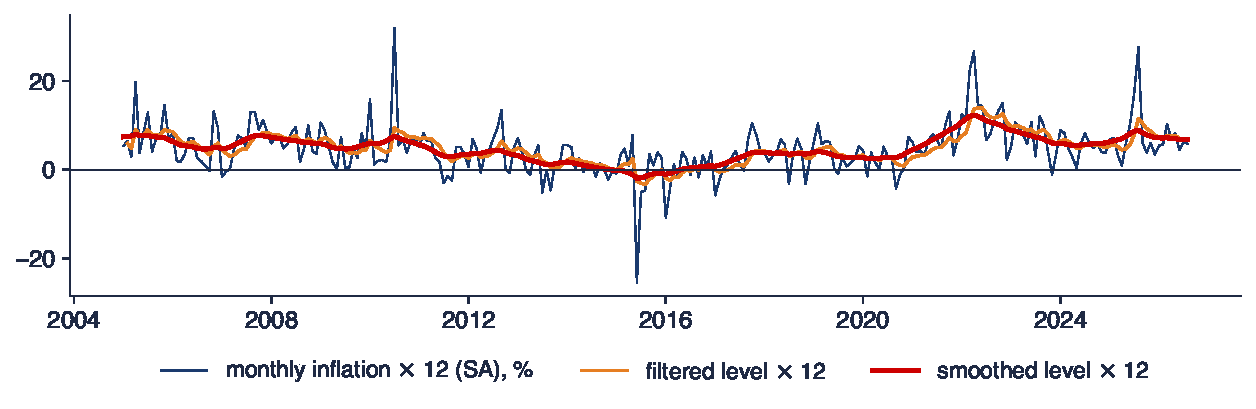
\includegraphics[width=0.96\textwidth,height=0.42\textheight,keepaspectratio]{ch10_sem_b1.pdf}
\end{center}
\vspace{-2mm}
\begin{itemize}
    \item $\hat\sigma^2_\varepsilon = 0{,}142$, $\hat\sigma^2_\eta = 0{,}0057$, $\hat q = 0{,}040$; $\bar K = 0{,}181$; SES prin cele mai mici pătrate: $\hat\alpha = 0{,}175$
    \item Nivelul netezit $\times 12$: maxim 12{,}3\% (aprilie 2022), minim \ensuremath{-}2{,}0\% (iunie 2015), ultima valoare 6{,}8\% (august 2026, SE 1{,}9); seria brută $\times 12$ are SD 5{,}6
    \item Interpretare: $q$ este mic: majoritatea mișcărilor lunare sînt zgomot (modificări de taxe, prețuri la alimente și energie); fiecare lună mută nivelul de fond cu aproximativ 0{,}181 din surpriză
\end{itemize}\quantlet{TSA\_ch10\_seminar}{\qlurl{TSA_ch10_seminar}}
\end{frame}

\begin{frame}{B2: deviația PIB a SUA [Propus]}
\itemsize{\footnotesize}
\begin{itemize}
\item \textbf{Întrebarea}: cît de aproape sînt trei deviații PIB statistice de deviația oficială a CBO și pe care ați folosi-o în timp real?
\item \textbf{Date}: PIB-ul real al SUA și PIB-ul potențial al CBO, trimestrial, 1949--2026; model: B1
\item \textbf{Cerințe}
\begin{enumerate}
    \item Calculați ciclul UC (trend neted plus AR(2)), deviația HP ($\lambda = 1600$) și filtrul Hamilton ($h = 8$, patru decalaje) pentru $100\log\mathrm{PIB}$.
    \item Calculați deviația CBO $100(\mathrm{PIB}/\mathrm{GDPPOT} - 1)$ și corelația fiecărei măsuri cu ea, inclusiv a ciclului UC filtrat.
    \item Raportați abaterile standard și ultimele valori.
    \item Interpretare: ce măsură ați folosi pentru a judeca economia astăzi?
\end{enumerate}
\item \textbf{Raportați}: cinci corelații, patru abateri standard, patru valori recente, o frază
\item Notebook: secțiunea B2
\end{itemize}
\end{frame}

\ifsolutions
\begin{frame}{B2: rezolvare [Propus]}
\itemsize{\scriptsize}
\begin{center}
\includegraphics[width=0.96\textwidth,height=0.42\textheight,keepaspectratio]{ch10_sem_b2.pdf}
\end{center}
\vspace{-2mm}
\begin{itemize}
    \item Corelația cu deviația CBO: UC netezit 0{,}77, UC filtrat 0{,}88, HP 0{,}78, Hamilton 0{,}72; SD: CBO 2{,}3, UC 2{,}9, HP 1{,}6, Hamilton 3{,}3
    \item Ultimele valori: CBO 1{,}4\%, UC 0{,}7\%, HP \ensuremath{-}0{,}4\%, Hamilton 0{,}5\%
    \item Interpretare: deviația HP este cea mai mică și este trasă spre zero la capătul eșantionului; pentru astăzi folosiți o măsură unilaterală (UC filtrat, Hamilton) și raportați-i incertitudinea
\end{itemize}\quantlet{TSA\_ch10\_seminar}{\qlurl{TSA_ch10_seminar}}
\end{frame}
\fi

\begin{frame}{B3: recesiunile în producția industrială din SUA [Rezolvat]}
\itemsize{\footnotesize}
\begin{itemize}
\item \textbf{Întrebarea}: găsește un model cu două regimuri pentru producția industrială recesiunile NBER?
\item \textbf{Date}: creșterea lunară a producției industriale din SUA, 1960--2019 (93 de luni de recesiune NBER)
\item \textbf{Cerințe}
\begin{enumerate}
    \item Estimați un model cu două regimuri, cu medie și varianță variabile (\texttt{MarkovRegression}).
    \item Raportați mediile și abaterile standard ale regimurilor, $p_{11}$, $p_{22}$ și duratele așteptate.
    \item Clasificați fiecare lună după probabilitatea netezită ($> 0{,}5$) și după cea filtrată și comparați cu lunile NBER.
    \item Interpretare: se potrivește regimul de recesiune cu recesiunile NBER?
\end{enumerate}
\item \textbf{Raportați}: șase parametri, două durate, două tabele de concordanță, o frază
\item Notebook: secțiunea B3
\end{itemize}
\end{frame}

\begin{frame}{B3: rezolvare [Rezolvat]}
\itemsize{\scriptsize}
\begin{center}
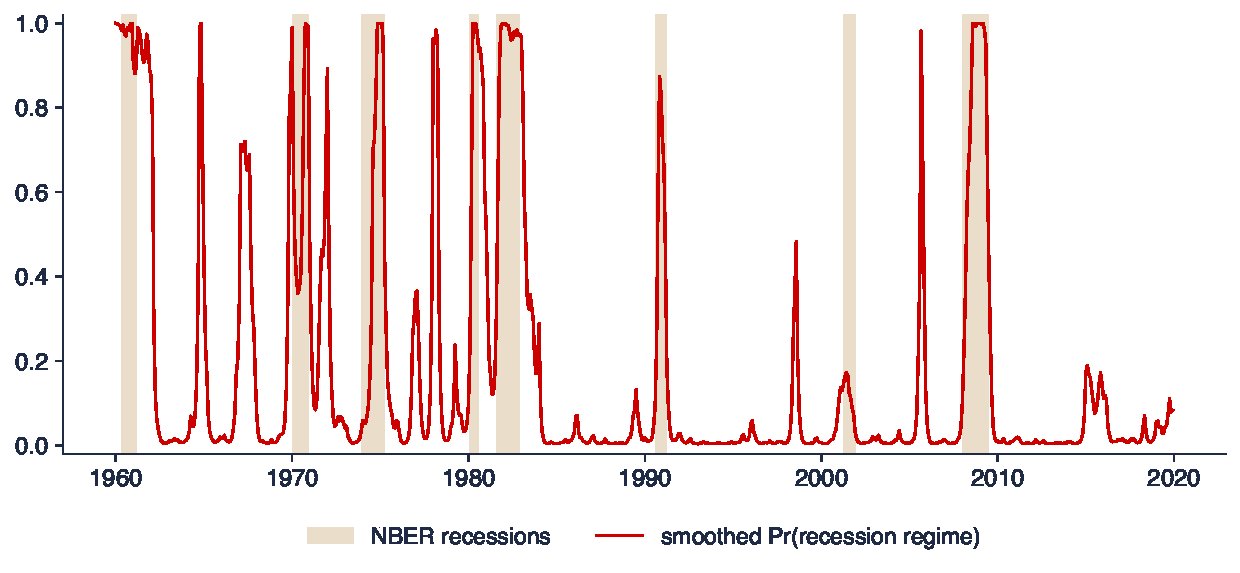
\includegraphics[width=0.96\textwidth,height=0.4\textheight,keepaspectratio]{ch10_sem_b3.pdf}
\end{center}
\vspace{-2mm}
\begin{itemize}
    \item Regimul de recesiune: media \ensuremath{-}0{,}16\%, SD 1{,}30; expansiunea: media 0{,}29\%, SD 0{,}51; $\hat p_{11} = 0{,}874$, $\hat p_{22} = 0{,}970$; durate de 8{,}0 și 33{,}2 luni; ponderea ergodică 19\%
    \item Netezit: 89\% din luni coincid, 69\% din lunile NBER găsite, 7\% alarme false; filtrat: 86\%, 57\%, 10\%
    \item Interpretare: da, pentru recesiunile profunde; regimul este „creștere scăzută și volatilă”, deci semnalează și unele încetiniri, iar în timp real găsește mai puține luni de recesiune
\end{itemize}\quantlet{TSA\_ch10\_seminar}{\qlurl{TSA_ch10_seminar}}
\end{frame}

\begin{frame}{B4: regimurile de volatilitate ale BET [Propus]}
\itemsize{\footnotesize}
\begin{itemize}
\item \textbf{Întrebarea}: are piața de la București regimuri calme și agitate și sînt ele aceleași cu cele ale S\&P 500?
\item \textbf{Date}: randamentele logaritmice săptămînale ale BET și S\&P 500, 2000--2026; model: B3
\item \textbf{Cerințe}
\begin{enumerate}
    \item Estimați un model cu două regimuri, cu medie și varianță variabile, pentru randamentele BET; raportați volatilitățile anualizate și duratele.
    \item Enumerați cei trei ani cu cea mai mare pondere de săptămîni agitate.
    \item Estimați un GARCH(1,1) (\tsachlink{https://danpele.github.io/Time-Series-Analysis/RO/Cursuri/capitol5_volatilitate_conditionata_garch.pdf}{Capitolul 5}) și corelați volatilitatea lui cu volatilitatea implicată de regimuri.
    \item Interpretare: sînt perioadele agitate ale BET aceleași cu cele ale S\&P 500?
\end{enumerate}
\item \textbf{Raportați}: două volatilități, două durate, trei ani, două corelații, o frază
\item Notebook: secțiunea B4
\end{itemize}
\end{frame}

\ifsolutions
\begin{frame}{B4: rezolvare [Propus]}
\itemsize{\scriptsize}
\begin{center}
\includegraphics[width=0.96\textwidth,height=0.4\textheight,keepaspectratio]{ch10_sem_b4.pdf}
\end{center}
\vspace{-2mm}
\begin{itemize}
    \item Calm: 14\% pe an, 33 de săptămîni; agitat: 40\% pe an, 12 săptămîni; agitat în 25\% din săptămîni; anii: 2009 (100\%), 2008 (94\%), 2001 (75\%)
    \item GARCH(1,1): $\alpha + \beta = 0{,}96$; corelația cu volatilitatea regimurilor 0{,}69; corelația probabilităților de regim agitat pentru BET și S\&P 500: 0{,}48 (aceeași clasificare în 78\% din săptămîni)
    \item Interpretare: doar parțial: crizele globale (2008--2009) sînt comune, dar BET are propriii ani agitați (2001--2002) și a fost mai ales calm în 2022 (27\% săptămîni agitate, față de 90\% pentru S\&P 500)
\end{itemize}\quantlet{TSA\_ch10\_seminar}{\qlurl{TSA_ch10_seminar}}
\end{frame}
\fi


%=============================================================================
\section{Partea C: întrebări deschise și critica unui răspuns AI}
%=============================================================================

\begin{frame}{C1: regimurile inflației din România [Propus]}
\itemsize{\footnotesize}
\begin{itemize}
\item \textbf{Întrebarea}: cîte regimuri de inflație a avut România din 1996 și cînd a început regimul de inflație scăzută?
\item \textbf{Date}: inflația lunară IAPC, neajustată sezonier, 1996--2026; țintirea inflației din august 2005; model: B3
\item \textbf{Cerințe}
\begin{enumerate}
    \item Estimați modele cu două și trei regimuri (medie și varianță variabile) și comparați-le după BIC.
    \item Pentru trei regimuri, raportați mediile, duratele și data de la care regimul scăzut devine permanent.
    \item Propuneți încă o verificare (sezonalitatea, un regim cu termen AR, prognoze în afara eșantionului).
    \item Interpretare: a declanșat țintirea inflației regimul de inflație scăzută?
\end{enumerate}
\item \textbf{Raportați}: șase parametri, o dată, o verificare și un plan de proiect
\item Notebook: secțiunea C1
\end{itemize}
\end{frame}

\ifsolutions
\begin{frame}{C1: analiză de referință [Propus]}
\itemsize{\scriptsize}
\begin{center}
\includegraphics[width=0.96\textwidth,height=0.42\textheight,keepaspectratio]{ch10_sem_c1.pdf}
\end{center}
\vspace{-2mm}
\begin{itemize}
    \item Medii (\% pe lună): scăzut 0{,}40 (SD 0{,}41, aproximativ 4{,}8\% pe an), mediu 2{,}20, ridicat 6{,}49; durate de 40{,}1; 7{,}8; 4{,}3 luni
    \item BIC: 910{,}8 cu două regimuri, 825{,}7 cu trei. Regimul scăzut apare în iulie 2002 și este regimul aproape tuturor lunilor din 2004, înainte de țintirea inflației; lunile de regim mediu revin în 2010, 2022 și iulie--august 2025 (majorările TVA din 2010 și 2025)
    \item Interpretare: dezinflația a început înainte de 2005; țintirea a consolidat-o. Proiect: adăugați un termen AR dependent de regim și comparați prognozele cu un model local level (B1)
\end{itemize}\quantlet{TSA\_ch10\_seminar}{\qlurl{TSA_ch10_seminar}}
\end{frame}
\fi

\begin{frame}{C2: verificați un răspuns AI [Propus]}
\itemsize{\scriptsize}
\begin{itemize}
    \item Un student a întrebat un asistent AI despre modelele în spațiul stărilor și cu regimuri. Răspunsul:
    \item \aiprompt{(a) Pentru Nil, q = 0,097, deci ponderea echivalentă de netezire exponențială este alpha = q = 0,097.}
    \item \aiprompt{(b) Cîștigul Kalman este K = sigma2\_eps / (P + sigma2\_eps): cu cît datele sînt mai zgomotoase, cu atît primesc o pondere mai mare.}
    \item \aiprompt{(c) Cu p11 = 0,75, recesiunile durează în medie p11 / (1 - p11) = 3 trimestre.}
    \item \aiprompt{(d) Pentru a anunța o recesiune în timp real, folosiți smoothed\_marginal\_probabilities din statsmodels.}
    \item \aiprompt{(e) Ultima valoare a deviației HP este o estimare de încredere a deviației PIB de azi.}
    \item \aiprompt{(f) În modelul local level prognozele pentru toate orizonturile sînt egale; doar varianța lor crește cu orizontul.}
    \item Cerințe
    \begin{itemize}
        \item 1. Pentru fiecare afirmație, precizați dacă este corectă; dacă nu este, formulați afirmația corectă și, acolo unde se poate, dați valoarea corectă (Partea A, secțiunea C2 din notebook).
        \item 2. Raportați: o listă de șase verdicte, fiecare cu un rînd de justificare.
    \end{itemize}
\end{itemize}
\end{frame}

\ifsolutions
\begin{frame}{C2: rezolvare [Propus]}
\itemsize{\scriptsize}
\begin{itemize}
    \item (a) Greșit: $\alpha = \bar K = 0{,}267$, nu $q$; relația este $q = \alpha^2/(1 - \alpha)$ (A3)
    \item (b) Greșit: $K = P/(P + \sigma^2_\varepsilon)$; datele zgomotoase primesc o pondere \textbf{mai mică} (A1)
    \item (c) Greșit: durata așteptată este $1/(1 - p_{11}) = 4$ trimestre (A5)
    \item (d) Greșit: probabilitățile netezite folosesc date viitoare; în timp real folosiți \texttt{filtered\_marginal\_probabilities} (B3)
    \item (e) Greșit: HP este bilateral, iar ultimele lui valori se revizuiesc cînd sosesc trimestre noi \refHamHP; folosiți o măsură unilaterală (B2)
    \item (f) Corect: $\hat y_{n+h} = a_{n+1}$ pentru orice $h$, cu varianța $P_{n+1} + (h - 1)\sigma^2_\eta + \sigma^2_\varepsilon$
\end{itemize}\quantlet{TSA\_ch10\_seminar}{\qlurl{TSA_ch10_seminar}}
\end{frame}
\fi


%=============================================================================
\section{Încheiere}
%=============================================================================

\begin{frame}{Idei de reținut}
\itemsize{\small}
\begin{itemize}
    \item Filtrul Kalman: $K_t = P_t/(P_t + \sigma^2_\varepsilon)$, $a_{t|t} = a_t + K_tv_t$; o valoare lipsă înseamnă fără actualizare
    \item Netezirea exponențială este un filtru local level în echilibru: $\alpha = \bar K$, $q = \alpha^2/(1 - \alpha)$
    \item Inflația lunară din România: $q$ mic, un nivel de fond care se mișcă lent
    \item Markov switching: durate $1/(1 - p_{ii})$; probabilitățile filtrate pentru timp real, cele netezite pentru istorie
    \item Un răspuns AI este o ciornă: verificați cîștigul, formula duratei, filtrat față de netezit
\end{itemize}
\end{frame}

\begin{frame}{După seminar}
\itemsize{\small}
\begin{itemize}
    \item Cursul 10 dezvoltă fiecare temă de azi: forma în spațiul stărilor, filtrul și netezitorul, verosimilitatea, trend și ciclu, modelele Markov switching
    \item Încercați cerințele [Propus] în notebook
    \item C1 poate deveni un proiect de echipă: regimurile inflației în România și în regiune
    \item Lectură: \refDK, cap.~2; \refHamMS; \refHamHP
    \item \textbf{Seminarul are rol de exercițiu și nu se notează; rezolvările cerințelor [Propus] se discută la seminar}
\end{itemize}
\end{frame}


%=============================================================================
\section{Bibliografie}
%=============================================================================

\begin{frame}{Bibliografie}
\itemsize{\tiny}
\begin{itemize}
    \item Durbin, J., \& Koopman, S. J. (2012). \textit{Time Series Analysis by State Space Methods} (2nd ed.). Oxford University Press. \href{https://doi.org/10.1093/acprof:oso/9780199641178.001.0001}{doi:10.1093/acprof:oso/9780199641178.001.0001}
    \item Hamilton, J. D. (1989). A new approach to the economic analysis of nonstationary time series and the business cycle. \textit{Econometrica}, 57(2), 357--384. \href{https://doi.org/10.2307/1912559}{doi:10.2307/1912559}
    \item Hamilton, J. D. (2018). Why you should never use the Hodrick--Prescott filter. \textit{The Review of Economics and Statistics}, 100(5), 831--843. \href{https://doi.org/10.1162/rest\_a\_00706}{doi:10.1162/rest\_a\_00706}
    \item Harvey, A. C. (1989). \textit{Forecasting, Structural Time Series Models and the Kalman Filter}. Cambridge University Press. \href{https://doi.org/10.1017/CBO9781107049994}{doi:10.1017/CBO9781107049994}
    \item Hodrick, R. J., \& Prescott, E. C. (1997). Postwar U.S. business cycles: An empirical investigation. \textit{Journal of Money, Credit and Banking}, 29(1), 1--16. \href{https://doi.org/10.2307/2953682}{doi:10.2307/2953682}
    \item Kalman, R. E. (1960). A new approach to linear filtering and prediction problems. \textit{Journal of Basic Engineering}, 82(1), 35--45. \href{https://doi.org/10.1115/1.3662552}{doi:10.1115/1.3662552}
    \item Muth, J. F. (1960). Optimal properties of exponentially weighted forecasts. \textit{Journal of the American Statistical Association}, 55(290), 299--306. \href{https://doi.org/10.1080/01621459.1960.10482064}{doi:10.1080/01621459.1960.10482064}
\end{itemize}
\end{frame}

\end{document}
